%]]] !LW recipe="pdflatex -> biber -> pdflatex * 2 "
%%%%%%%%%%%%%%%%%%%%%%%%%%%%%%%%%%%%%%%%%%%%%%%%%%%%%%%%%%%%%%%%%%%%%%%%%%%%%%
% University of Bristol presentation theme based on the PowerPoint template
%
% Copyright (c) 2012, 2020 David A.W. Barton (david.barton@bristol.ac.uk)
% All rights reserved.
%
% The latest version of this theme can be found at
%   https://github.com/db9052/UoB-beamer-theme
%
% This is dual licensed under the MIT license and CC BY 4.0
%%%%%%%%%%%%%%%%%%%%%%%%%%%%%%%%%%%%%%%%%%%%%%%%%%%%%%%%%%%%%%%%%%%%%%%%%%%%%%
% \documentclass[aspectratio=169, handout]{beamer}
\documentclass[aspectratio=169]{beamer}
    % Possible aspect ratios are 16:9, 16:10, 14:9, 5:4, 4:3 (default) and 3:2
    % (Remember to remove the colon, i.e., 16:9 becomes the option 169) 

% \bibliographystyle{apalike}

\beamertemplatenavigationsymbolsempty % Remove navigation symbols

\usepackage{tikz}
%\usetikzlibrary{shapes,arrows,positioning}
\usetikzlibrary{automata,arrows,positioning,calc}
\usetikzlibrary{shapes,snakes}

\usepackage{amsmath}
\usepackage{amssymb}
\usepackage{bm}
\usepackage{dsfont}

\usepackage{mathtools}
\newcommand{\defeq}{\vcentcolon=}
\newcommand{\eqdef}{=\vcentcolon}
\newcommand{\Var}{\text{Var}}
% \renewcommand{\bm{\Sigma}}{\bm{\bm{\Sigma}}}

\DeclareMathOperator*{\argmax}{argmax} % thin space, limits underneath in displays
\DeclareMathOperator*{\argmin}{argmin}

%%%%%%%%%%%%%%%%%%%%%%%%%%%%%%%%%%%%%%%%%%%%%%%%%%%%%%%%%%%%%%%%%%%%%%%%%%%%%%
\title[Short Title]{Adaptive MCMC}
% \subtitle{Filtering, Smoothing \& Parameter Estimation}
\author{}%Sam Bowyer}
\date{5th July 2023}

%%%%%%%%%%%%%%%%%%%%%%%%%%%%%%%%%%%%%%%%%%%%%%%%%%%%%%%%%%%%%%%%%%%%%%%%%%%%%%
% Lectures to include

% Lectures available (see \lecture commands below):
%   01: Introductory slides

\ifdefined\uselecture
  % Automatically generate specific lecture slides: run (lua/pdf)latex with
  % latex -jobname "slides-01" "\def\uselecture{01}\documentclass[aspectratio=169]{beamer}
% \documentclass[aspectratio=169, handout]{beamer}

\usetheme{Madrid}
\usecolortheme{beaver}

\usepackage{graphicx}
\usepackage{amsmath}
\usepackage{amssymb}
\usepackage{amsthm}
\usepackage{mathrsfs}
\usepackage{hyperref}

\usepackage{tikz}
\usetikzlibrary{bayesnet}
\usetikzlibrary{arrows}


% \usepackage{graphicx}
% \usepackage{booktabs}
% \usepackage{pgfplots}
% \pgfplotsset{compat=1.14}
% \usepackage{anyfontsize}
% % \usepackage{minted}
% \usepackage[cache=false]{minted} 
% \setminted[python]{
%     linenos,
%     % bgcolor=LightGray,
%     % breaklines,
%     fontsize=\scriptsize,
%     % xleftmargin=1.1em,
%     numbersep=4pt
% }

% \usepackage{tcolorbox}

% \newtcolorbox[auto counter]{pbox}[2][]{
%   colback=white,
%   title=#2,
%   #1,
%   fonttitle= \large, %\sffamily,
%   % fontupper=\sffamily,
%   boxrule=0.5pt, 
%   arc=2pt,
%   top=1pt, 
%   bottom=1pt,
%   before={\vspace{2pt}}, 
%   after={\vspace{2pt}} 
%   % colframe=..,
%   % coltitle=..,
%   % colbacktitle=..,
%   % toptitle=0.05cm,
%   % bottomtitle=0.125cm
% }

% \usepackage{fancyvrb}


\setbeamertemplate{caption}{%
  \raggedright
  \insertcaption\par
}

\usepackage[style=authoryear, autocite=footnote, backend=biber]{biblatex}
\addbibresource{refs.bib}

\title[Cohere Research Talk]{Cohere Research Talk: Massively Parallel Inference \& Bayesian Evals}
\author{Sam Bowyer}
\date{November 2025}

\begin{document}

\begin{frame}
  \titlepage
\end{frame}

\begin{frame}{Outline}
  \tableofcontents
\end{frame}

% --- Part 1: Overview ---
\section{About Me}

\begin{frame}{About Me}
  \begin{itemize}[<+->] 
    \item Fourth (final) year PhD student at Bristol's Compass CDT (Computational Statistics and Data Science).
    \item Based in the School of Maths, but supervised by Laurence Aitchison (CS/Engineering Maths), Mengyue Yang (Engineering Maths), and Song Liu (Maths).
    \item Currently working on discrete diffusion models (training an `auxilliary' model with VI to suggest the order in which to decode tokens).
    % \item Also worked on RL and LoRA finetuning.
    \item Two projects I'll be talking about today: Alan (massively parallel probabilistic programming) \& Bayesian Evals.
  \end{itemize}
\end{frame}


% --- Part 2: Alan, Massively Parallel Inference ---
\section{Alan: Massively Parallel Probabilistic Programming}


\begin{frame}{Alan: A Massively Parallel Probabilistic Programming Language}
  \begin{figure}
    \centering
    \includegraphics[height=0.25\textheight]{img/laurence.png}
    \includegraphics[height=0.25\textheight]{img/thomas.png}
    \includegraphics[height=0.25\textheight]{img/sam.png}
    \caption{Work done with Laurence Aitchison and Thomas Heap over the first two years of my PhD.}
  \end{figure}
  \pause
  \begin{itemize}[<+->]
    % \item Work with Laurence Aitchison and Thomas Heap over the first two years of my PhD.
    \item Dual goals:
      \begin{itemize}
        \item Develop `massively parallel' Bayesian inference algorithms: fast, accurate, and scalable; desinged for GPU acceleration.
        \item Implement these algorithms in a probabilistic programming language in pytorch (\texttt{alan}), allowing users to specify general probabilistic models.
      \end{itemize}
  \end{itemize}
\end{frame}


\begin{frame}{Regular Bayesian Inference}
  \begin{itemize}[<+->]
    \item \textbf{Bayesian inference}: Prior $P(z)$ and likelihood $P(x|z)$ for latent variables $z$ and data $x$.
      $$P(z|x) = \frac{P(x|z)P(z)}{\int_\mathcal{Z} P(x,z') dz'}$$
    \item \textbf{Importance sampling}: 
      \begin{enumerate}
        \item Sample $K$ latent variables from a proposal distribution $Q$ (usually IID):
          $$z = (z^1, \ldots, z^K) \sim Q(z).$$ 
        \item Compute importance weights: 
          $$r_k(z) = \frac{P(x , z^k)}{Q(z^k)}.$$ 
        \item Approximate the normalising constant using the `global' estimator: 
          $$\mathcal{P}_\text{global}(z) = \frac{1}{K} \sum_{k=1}^K r_k(z) \quad \text{such that } \quad \mathbb{E}_{z \sim Q}[\mathcal{P}_\text{global}(z)] = P(x).$$ 
      \end{enumerate}
  \end{itemize}
\end{frame}

\begin{frame}{Limitations of Importance Sampling (IS)}
  \begin{itemize}[<+->]
    \item Global IS scales poorly with the number of latent variables, $n$.
    \begin{itemize}
      \item $z^k = (z_1^k, \ldots, z_n^k) \in \mathcal{Z}$.
      % \item E.g. $n$ is the dimension of $z$ if all latent variables are scalar.
    \end{itemize} 
    \item Chatterjee \& Diaconis (2018) show that as $n$ increases, the number of samples, $K$, must increase with $O(e^{D_{\text{KL}}(P(z|x) || Q(z))}) \approx O(e^n)$. (This is a lot!)
    \item Solution: \textbf{Massively Parallel Importance Sampling (MP-IS)}
      \begin{itemize}
        \item Reason about all $K^n$ possible joint samples at once.
      \end{itemize}
  \end{itemize}
\end{frame}


\begin{frame}{Massively Parallel Importance Sampling (MP-IS)}
  \begin{minipage}{0.55\textwidth}
    \begin{figure}
      \includegraphics[width=\textwidth]{img/alan/MPIS.pdf}
    \end{figure}
  \end{minipage}
  \begin{minipage}{0.43\textwidth}
    \begin{itemize}[<+->]
      \item Suppose each latent sample $z^k = (z_1^k, \ldots, z_n^k) \sim Q(z)$ is comprised of $n$ variables.
      \item We can construct $K^n$ different samples from the full joint space 
      $$(z_1^{k_1}, \ldots, z_n^{k_n}) \in \mathcal{Z}$$
      where $\mathbf{k} = (k_1, \ldots, k_n) \in [K]^n$ is the indexing vector for each latent variable.
    \end{itemize}
  \end{minipage}
\end{frame}

\begin{frame}{Massively Parallel Importance Sampling (MP-IS)}
  \begin{minipage}{0.55\textwidth}
    \begin{figure}
      \includegraphics[width=\textwidth]{img/alan/MPIS.pdf}
    \end{figure}
  \end{minipage}
  \begin{minipage}{0.43\textwidth}
    \begin{itemize}[<+->]
      \item Rather than using the global IS estimator
      $$\mathcal{P}_\text{global}(z) = \frac{1}{K} \sum_{k=1}^K \frac{P(x, z^k)}{Q(z^k)}.$$
      \item ...we can use the MP-IS estimator
      $$\mathcal{P}_\text{MP}(z) = \frac{1}{K^n} \sum_{\mathbf{k}\in [K]^n} \frac{P(x, z^\mathbf{k})}{Q_\text{MP}(z^\mathbf{k}, \mathbf{k})}.$$
      (Which is still unbiased.)
    \end{itemize}
  \end{minipage}
\end{frame}

% \begin{frame}{MP-IS: Some Complications...}
%   $$\mathcal{P}_\text{MP}(z) = \frac{1}{K^n} \sum_{\mathbf{k}\in [K]^n} \frac{P(x, z^\mathbf{k})}{Q_\text{MP}(z^\mathbf{k}, \mathbf{k})}.$$
%   \begin{itemize}[<+->]
%     \item We have to be careful about how we define $Q_\text{MP}$ over the space of all $K^n$ joint samples.
%     \item We can use a hierarchical model:
%       $$Q_\text{MP}(z, \mathbf{k}) = \prod_{i=1}^n Q_\text{MP}(z_i^{k_i} | z_j \text{ for } j \in \text{qa}(i)),$$
%       where $\text{qa}(i)$ is the set of indices of parents of $z_i$ in the proposal model.
%     \item If variable $z_i$ has a parent samples $z_j = (z_j^1, \ldots, z_j^K) \sim Q(z_j)$, then we can sample $z_i^{k_i}$ from $Q(z_i^{k_i} | z_j^{\pi(k_i)})$ for a (uniformly) random permutation $\pi$ of $[K]$.  \end{itemize}
% \end{frame}

\begin{frame}{MP-IS: Some Complications...}
  $$\mathcal{P}_\text{MP}(z) = \frac{1}{K^n} \sum_{\mathbf{k}\in [K]^n} \frac{P(x, z^\mathbf{k})}{Q_\text{MP}(z^\mathbf{k}, \mathbf{k})} = \frac{1}{K^n} \sum_{\mathbf{k}\in [K]^n} r_\mathbf{k}(z).$$

  \begin{itemize}[<+->]
    \item We have to be careful about how we define $Q_\text{MP}$ over the space of all $K^n$ joint samples.
    \item Also, at first glance, this thing doesn't look all that nice to compute...
    \item But we can exploit the conditional independencies in the model to render it tractable.
  \end{itemize}

\end{frame}


\begin{frame}{MP-IS: Some Complications...}

  \begin{figure}
    \includegraphics[width=0.6\textwidth]{img/alan/toy_model.drawio.pdf}
  \end{figure}

  \begin{itemize}[<+->]
    \item E.g. with the model from before with $n=3$, $P(x, z) =  P(z_1) P(z_2 | z_1) P(z_3 | z_2) P(x | z_3)$, we can move the sums inside the product and get a bunch of tensor products:
  \end{itemize}
    \pause
    $$
    % \begin{aligned}
      \mathcal{P}_\text{MP}(z) = \frac{1}{K^3} \sum_{k_1 \in [K]} \sum_{k_2 \in [K]} \sum_{k_3 \in [K]} \frac{P(z_1^{k_1}) P(z_2^{k_2} | z_1^{k_1}) P(z_3^{k_3} | z_2^{k_2}) P(x | z_3^{k_3})}{Q(z_1^{k_1}) Q(z_2^{k_2}) Q(z_3^{k_3})}
      % = \frac{1}{K^3} \sum_{k_1 \in [K]} \sum_{k_2 \in [K]} \sum_{k_3 \in [K]} r_{k_1,k_2,k_3}(z)
    $$
    \pause
    $$
      = \frac{1}{K^3} \sum_{k_1 \in [K]} \underbrace{\frac{P(z_1^{k_1})}{Q(z_1^{k_1})}}_{\text{Vector of size } K} 
      \sum_{k_2 \in [K]} \underbrace{\frac{P(z_2^{k_2} | z_1^{k_1})}{Q(z_2^{k_2})}}_{\text{Matrix of size } K \times K}
      \sum_{k_3 \in [K]} \underbrace{\frac{P(z_3^{k_3} | z_2^{k_2})}{Q(z_3^{k_3})}}_{\text{Matrix of size } K \times K}
      \underbrace{P(x | z_3^{k_3})}_{\text{Vector of size } K}
    % \end{aligned}
    $$
    % \item This can be computed efficiently on a GPU using tensor operations.
  % \end{itemize}
\end{frame}


\begin{frame}{Can we hide these complications from the user?}
  \begin{itemize}[<+->]
    \item Yes! We do this with \texttt{alan}.
    \item User specifies the model with P and Q as pytorch modules, and we handle the massively parallel inference for them.
  \end{itemize}
\end{frame}

\begin{frame}{Alan: A Probabilistic Programming Language}

  \begin{minipage}{0.7\textwidth}
    \begin{figure}
      \centering
      \includegraphics[width=0.9\textwidth]{img/alan/movielens_code_1.png}
    \end{figure}
  \end{minipage}
  \begin{minipage}{0.25\textwidth}
    % \vspace{-1cm}
    \begin{figure}[t]
      \centering
      \resizebox{0.8\textwidth}{!}{%
        \tikz{
          % nodes
           \node[obs] (rating) {\(\mathrm{Rating}_{mn}\)};%
           \node[latent,above=of rating] (peruser) {\(\mathbf{z}_m\)}; %
           \node[latent, above=of peruser, xshift=-1cm] (psi) {\(\boldsymbol{\psi}\)};
          \node[latent, above=of peruser, xshift=1cm] (mu) {\(\boldsymbol{\mu}\)};
          % plate
           \plate [inner sep=.3cm] {plate2} {(rating)} {\(\mathrm{N}\) Films}; %
           \plate [inner sep=.3cm] {plate1} {(peruser)(plate2)} {\(\mathrm{M}\) Users}; %
          edges
           \edge {psi,mu} {peruser}
           \edge {peruser} {rating}}
           }
    \end{figure}
  \end{minipage}

\end{frame}

\begin{frame}{MP-VI}
  \begin{itemize}[<+->]
    \item Using $\mathcal{P}_\text{MP}(z)$, we can do variational inference (VI) by maximising the ELBO:
      $$
      \log P(x) \geq \mathcal{L}_\text{MP}(\theta) = \mathbb{E}_{z \sim Q_\text{MP}(\theta)}[\log \mathcal{P}_\text{MP}(z)]
      $$
    \item Aitchison (2019) showed that MP-VI is a tighter bound than the global VI objective (IWAE):
      $$
      \log P(x) \geq \mathcal{L}_\text{MP}(\theta) \geq \mathcal{L}_\text{global}(\theta) = \mathbb{E}_{z \sim Q(\theta)}[\log \mathcal{P}_\text{global}(z)]
      $$
  \end{itemize}
  \pause
  \begin{figure}
    \centering
    \includegraphics[width=0.9\textwidth]{img/alan/movielens_code_2.png}
  \end{figure}
\end{frame}

\begin{frame}{MP Algorithms}
  \begin{itemize}[<+->]
    \item We can obtain unbiased posterior moment estimates via autodiff (Bowyer et al. (2024)).
      $$
      m_\text{MP}(z) = \frac{1}{K^n} \sum_{\mathbf{k} \in [K]^n} \frac{r_\mathbf{k}(z)}{\mathcal{P}_\text{MP}(z)}m(z^\mathbf{k})
      $$
    \item We define a modified marginal likelihood estimator with an auxiliary variable $J \in \mathbb{R}$:
      $$
      \mathcal{P}_\text{MP}^\text{exp}(z, J) = \frac{1}{K^n} \sum_{\mathbf{k} \in [K]^n} r_\mathbf{k}(z) \exp(J m(z^\mathbf{k}))
      $$
    \item Then differentiating the log of this with respect to $J$ and setting $J=0$ we get:
      $$
      \frac{\partial}{\partial J}\bigg|_{J=0} \log \mathcal{P}_\text{MP}^\text{exp} (z, J) = \frac{\frac{\partial}{\partial J}\bigg|_{J=0} \mathcal{P}_\text{MP}^\text{exp} (z, J)}{\mathcal{P}_\text{MP}^\text{exp} (z, 0)} = m_\text{MP}(z)
      $$
    \item By similar arguments: $J \in \mathbb{R}^K$ gives us marginal importance weights; $J \in \mathbb{R}^{K^{1+|pa(i)|}}$ gives us importance samples for $z_i$, given its parents $pa(i)$.
  \end{itemize}
  \vspace{0.1cm}
\end{frame}

\begin{frame}{QEM: An Adaptive Importance Sampling Algorithm}
  \begin{minipage}{0.4\textwidth}
    \textbf{QEM} (Heap et al. (2025))
    \begin{enumerate}
      \item Start with an initial approximate posterior $Q_0$.
      \item Compute posterior moment estimates $m_\text{MP}(z)$ using MP-IS.
      \item Update the approximate posterior $Q_{t+1}$ using the moment estimates.
    \end{enumerate}    
  
    Can be seen as an EM-like algorithm for adaptive imortance sampling.
  \end{minipage}
  \begin{minipage}{0.59\textwidth}
    \begin{figure}
      \centering
      \includegraphics[width=0.95\textwidth]{img/alan/QEM_results.pdf}
    \end{figure}
  \end{minipage}
\end{frame}

\begin{frame}{Conclusions}
  \begin{itemize}[<+->]
    \item This project was a great (if, at times, complicated) way to learn about Bayesian inference and numerical and probabilistic programming.
    \item The results were pretty promising, but but there are some drawbacks to massively parallel methods:
    \begin{itemize}
      \item The algorithms are complex to implement (hence wrapping them in a PPL).
      \item Not all models have lots of conditional independencies to exploit.
      \item Although it's slower and harder to tune, HMC is often hard to beat in terms of quality of inference.
    \end{itemize}
  \end{itemize}
\end{frame}

% --- Part 3: Bayesian Evals, Uncertainty Quantification for LLM Evals ---
\section{Bayesian Evals: Uncertainty Quantification for LLM Evals}

\begin{frame}{Bayesian Evals: Uncertainty Quantification for LLM Evals}
  \begin{figure}
    \centering
    \includegraphics[height=0.25\textheight]{img/laurence.png}
    \includegraphics[height=0.25\textheight]{img/desi.jpg}
    \includegraphics[height=0.25\textheight]{img/sam.png}
    \caption{Work done with Laurence Aitchison and Desi R. Ivanova.}
  \end{figure}
  \begin{itemize}[<+->]
    \item Two directions:
      \begin{itemize}
        \item Improved UQ for evals with Bayesian methods.
        \item Interpretability of evals with Bayesian hierarchical modelling and SAE-like approaches.
      \end{itemize}
    \item The former direction led to an ICML spotlight position paper: \emph{`Position: Don't Use the CLT in LLM Evals With Fewer Than a Few Hundred Datapoints'}.
    \item The latter fell by the wayside, but is something I'd like to come back to at some point.
  \end{itemize}
\end{frame}

% --- Slide 2: Motivation ---
\begin{frame}{Motivation}
  \begin{block}{Central Limit Theorem (CLT)}
    If $X_1, \dots, X_N$ are IID r.v.s with mean $\mu \in \mathbb{R}$ and finite variance $\sigma^2$, then 
    $$
      \sqrt{N} (\hat{\mu} - \mu) \xrightarrow{d} \mathcal{N}( 0, \sigma^2 ) \; \text{as } N \rightarrow \infty,
    $$
    where $\hat{\mu} = \frac{1}{N}\sum_{i=1}^N X_i$ is the sample mean.
  \end{block}
  \pause
  \begin{itemize}[<+->]
      % \item Error bars are important for interpreting evals.
      \item The CLT-based confidence interval is:
      $$
        \text{CI}_{1-\alpha}(\mu) = \hat{\mu} \pm z_{\alpha/2} \text{SE}(\hat{\mu})
      $$
      where $z_{\alpha/2}$ is the $100(1-\alpha/2)$-th percentile of $\mathcal{N}(0, 1)$ and $\text{SE}(\hat{\mu}) = \sqrt{\frac{\hat{\sigma}^2}{N}}$ is the standard error of the sample mean.
      \item In the case of binary data $X_i \in \{0, 1\}$, this becomes:
      $$
        \text{CI}_{1-\alpha}(\theta) = \bar{X} \pm z_{\alpha/2} \sqrt{\bar{X}(1-\bar{X})/N}.
      $$
  \end{itemize}
  
\end{frame}

\begin{frame}{Real-World Failures of the CLT}
  \begin{itemize}[<+->]
    \item If $N$ is too small, CLT-based error bars can collapse to \alert{zero-width} or \alert{extend past $[0,1]$}.
    \item Smaller, more intricate, and expensive LLM benchmarks are becoming increasingly common, so we need to find alternatives for the few-data regime.
  \end{itemize}
  % \vspace{0.5cm}
  \begin{minipage}{0.45\textwidth}
    \centering
    \begin{figure}
      \includegraphics[height=4.2cm, keepaspectratio]{img/bayes_evals/pngs/real_data_matharena_aime_II_subset.png}
      \caption{Math Arena's AIME II 2025 Benchmark (N=15). Various 95\% interval types shown.}
    \end{figure}
  \end{minipage}
  \begin{minipage}{0.45\textwidth}
    \centering
    \begin{figure}
        \includegraphics[height=4.2cm, keepaspectratio]{img/bayes_evals/langchain_clt.png}
        \caption{Langchain Typewriter Tool Use Benchmark (N=20). CLT-based 95\% intervals only.}
    \end{figure}
  \end{minipage}
\end{frame}

% --- Slide 3: Bayesian Alternative -- Beta-Bernoulli Model ---
\begin{frame}{Bayesian Alternative: Beta-Binomial Model}
  \begin{itemize}[<+->]
    \item Treat the data as IID Bernoulli with a \alert{uniform prior} on the parameter $\theta$.
    $$
      \begin{aligned}
      \theta &\sim \text{Beta}(1, 1) = \text{Uniform}[0, 1] \\
      y_i &\sim \text{Bernoulli}(\theta) \; \text{for } i=1,\dots N 
      \end{aligned}
    $$
    \item Say $y_i$ is correct if $y_i = 1$ and incorrect if $y_i = 0$. %(Think of $\theta$ as the probability of correctness.)  
    \item Obtain quantile-based Bayesian \alert{credible intervals} for $\theta$ from the closed form posterior.
    $$
      p(\theta | y_{1:N}) = \text{Beta}\left(1+\sum_{i=1}^N y_i, 1 + \sum_{i=1}^N (1-y_i)\right)
    $$

  \end{itemize}
  
\pause
\begin{figure}
  \centering
  \includegraphics[width=0.8\textwidth]{img/bayes_evals/bayes_evals_code1.png}
\end{figure}


% \begin{pbox}[label={ex:bayes_simple}]{Beta-Bernoulli Bayesian Credible Interval}
%   \begin{minted}[fontsize=\scriptsize,breaklines]{python}
%  y is a length N binary "eval" vector
% S, N = y.sum(), len(y)  total successes & questions

% # Bayesian Credible interval
% posterior = scipy.stats.beta(1 + sum(y), 1 + N - sum(y))
% bayes_ci  = posterior.interval(confidence=0.95)
%   \end{minted}
% \end{pbox}

\end{frame}

% --- Slide 4: Frequentist Alternatives ---
\begin{frame}{Frequentist Alternatives}
  % \vspace{1cm}
  \begin{itemize}[<+->]
      \item \alert{Wilson score interval}: Based on normal approximation to the binomial distribution.
        \pause
        $$ \text{CI}_{1-\alpha, \text{Wilson}}(\theta) = \frac{\hat{\theta} + \frac{z_{\alpha/2}^2}{2N}}{1 + \frac{z_{\alpha/2}^2}{N}} \pm \frac{\frac{z_{\alpha/2}}{2N}}{1 + \frac{z_{\alpha/2}^2}{N}}\sqrt{4N\hat{\theta}(1 - \hat{\theta}) + z_{\alpha/2}^2} $$
        \pause
      \item \alert{Clopper-Pearson `exact' interval}: A `worst-case' approach; very conservative method guaranteed to never under-cover.
      $\text{CI}_{1-\alpha, \text{CP}}(\theta) = [\theta_\text{lower}, \theta_\text{upper}]$, 
        \pause
        $$ \theta_\text{lower} = B\left(\frac{\alpha}{2}, \sum_{i=1}^N y_i, 1+\sum_{i=1}^N(1-y_i)\right) \; \text{and} \; \theta_\text{upper} = B\left(1-\frac{\alpha}{2}, 1+ \sum_{i=1}^N y_i, \sum_{i=1}^N(1-y_i)\right) $$
        where $B(\alpha, a, b)$ is the $\alpha$-th quantile of the Beta$(a, b)$ distribution.
  \end{itemize}
  
  \pause
  % \vspace{1cm}
  % Implementation using \texttt{scipy}:
%   \begin{verbatim}
% # y is a length N binary "eval" vector
% S, N = y.sum(), len(y) # total successes & questions
% result = scipy.stats.binomtest(k=S, n=N)

% # 95% Wilson score interval and Clopper-Pearson exact interval
% wilson_ci = result.proportion_ci("wilson", 0.95)
% cp_ci = result.proportion_ci("exact", 0.95)
%   \end{verbatim}
\begin{figure}
  \centering
  \includegraphics[width=0.8\textwidth]{img/bayes_evals/bayes_evals_code2.png}
\end{figure}
\end{frame}

% --- Slide 5: Interval Comparison Simulations ---
\begin{frame}{Interval Comparison Simulations}
  \vspace{1cm}
  We use synthetic eval data so that we \alert{know} the true parameter $\theta$.
  
  \begin{itemize}[<+->]
      \item Draw $\theta \sim \text{Uniform}[0, 1]$.
      \item Draw $N \in \{3,10,30,100\}$ IID Bernoulli datapoints with parameter $\theta$.
      \item Construct intervals with various methods for various $1-\alpha$ confidence levels.
      \item Repeat many times and calculate the true coverage and average width of the intervals.
      \begin{itemize}
        \item Coverage: What proportion of the time does a $1-\alpha$ confidence-level interval \alert{actually contain} the true parameter? (A frequentist metric, really.)
        \item Ideally, $\text{coverage} = 1-\alpha$.
      \end{itemize}
  \end{itemize}
\end{frame}

% --- Slide 6: IID Questions Setting ---
\begin{frame}{IID Questions Setting: Results}
  \begin{figure}
      \includegraphics[width=\textwidth, height=0.8\textheight, keepaspectratio]{img/bayes_evals/fig/exp4-1_top_row_only.pdf}
      % \caption{Simulation results comparing Coverage and Width for different $N$.}
  \end{figure}
\end{frame}

\begin{frame}{IID Questions Setting: Results}
  \begin{figure}
      \includegraphics[width=\textwidth, height=0.8\textheight, keepaspectratio]{img/bayes_evals/fig/exp4-1_inkscape.pdf}
      % \caption{Simulation results comparing Coverage and Width for different $N$.}
  \end{figure}
\end{frame}

% --- Slide 7: Other Eval Settings ---
\begin{frame}{Other Eval Settings}
  \begin{itemize}[<+->]
      \item \textbf{Clustered Questions}
      \begin{itemize}
          \item Instead of $N$ IID questions, we have $T$ tasks, each with $N_t$ IID questions.
      \end{itemize}
      
      \item \textbf{Comparisons Between Two Models, $\theta_A$ and $\theta_B$}
      \begin{itemize}
          \item Independent Comparisons (using $N_A, N_B, \bar{y}_A, \bar{y}_B$ only).
          \item Paired Comparisons (using $N_A = N_B, \{y_{A;i}\}_{i=1}^N, \{y_{B;i}\}_{i=1}^N$).
          % \item Hypothesis testing $H_0: \theta_A = \theta_B$ vs $H_1: \theta_A > \theta_B$.
          \item With Bayes you can calculate $\mathbb{P}(\theta_A > \theta_B | y_A, y_B)$.
      \end{itemize}
      
      \item \textbf{Metrics that aren't simple averages of binary results} (e.g. F1 score).
      
      \item \textbf{Prior Mismatch} (i.e. what if the uniform prior is incorrect, $\theta \nsim \text{Uniform}[0, 1]$?).
  \end{itemize}
\end{frame}


% --- Slide 8: Clustered Questions Setting ---
\begin{frame}{Clustered Questions Setting: Frequentist Approach}
  \begin{itemize}[<+->]
    \item Instead of $N$ IID questions, we have $T$ tasks, each with $N_t$ IID questions.
    \item Some tasks are easier than others.% (e.g. each task asks $N_t$ questions about a single piece of input text, with texts varying in difficulty).
    \item Frequentist approach (Miller, 2024):
    $$
    \text{CI}_{1-\alpha}(\theta) = \bar{X} \pm z_{\alpha/2} \text{SE}_\text{Clustered}
    $$
    $$
    \text{SE}_\text{Clustered} = \sqrt{\text{SE}_\text{CLT}^2 + \frac{1}{N^2}\sum_{t=1}^T \sum_{i=1}^{N_t} \sum_{j \neq i} (y_{i,t} - \bar{y})(y_{j,t} - \bar{y})}
    $$
    % \item An improved standard error, but fundamentally still using the CLT.
  \end{itemize}
\end{frame}


\begin{frame}{Clustered Questions Setting: A Bayesian Approach}
  \begin{itemize}[<+->]
    \item `Dispersion' parameter $d$ controls the range of difficulty across tasks,
    $$d \sim \text{Gamma}(1, 1).$$
    \item $\theta$ is the mean difficulty of the questions across tasks,
    $$
    \theta \sim \text{Beta}(1, 1) = \text{Uniform}[0, 1].
    $$
    \item $\theta_t$ is the difficulty of the questions in task $t$ (we ensure that $\mathbb{E}[\theta_t | \theta] = \theta$),
    $$  
    \theta_t \sim \text{Beta}(d \theta, d (1-\theta)).
    $$
    \item $\text{Var}(\theta_t | \theta) = \frac{\theta (1-\theta)}{d^2 + 1}$.
    \item If $d$ is large, then $\theta_t$ is close to $\theta$ for all tasks.
    \item If $d$ is small, then $\theta_t$ is more variable across tasks.
  \end{itemize}
\end{frame}

\begin{frame}{Clustered Questions Setting: A Bayesian Approach}
  \vspace{-0.5cm}
  $$
    \begin{aligned}
    d &\sim \text{Gamma}(1, 1), \quad 
    \theta \sim \text{Beta}(1, 1), \quad 
    \theta_t &\sim \text{Beta}(d \theta, d (1-\theta)), \quad
    y_{i,t} \sim \text{Bernoulli}(\theta_t)
    \end{aligned}
  $$
  \vspace{-0.5cm}
  \pause
  \begin{itemize}[<+->]
    \item Can we integrate out the per-task difficulty parameters $\theta_t$?
    \item Yes! The number of successes per task is \alert{Beta-Binomial} distributed: 
      $$
        \sum_{i=1}^{N_t} y_{i,t} = Y_t \sim \text{BetaBinomial}(N_t, d \theta, d (1-\theta)).
      $$
    \item Get an \alert{importance-weighted posterior} for $\theta$: draw prior samples $\{(\theta^{(k)}, d^{(k)})\}_{k=1}^K$, then compute weights
      $$
        w^{(k)} = \prod_{t=1}^T p(Y_t | \theta^{(k)}, d^{(k)}).
      $$
    \item Compute quantile-based Bayesian credible intervals for $\theta$.
  \end{itemize}
\end{frame}

\begin{frame}{Clustered Questions Setting: Results}
  \begin{figure}
      \includegraphics[width=\textwidth, height=0.8\textheight, keepaspectratio]{img/bayes_evals/pngs/exp4-2.png}
      % \caption{Simulation results comparing Coverage and Width for different $N$.}
  \end{figure}
\end{frame}


% --- Slide 9: Conclusion ---
\begin{frame}{Conclusion}
  Advice to practitioners:
  
  \begin{itemize}[<+->]
      \item Use \alert{Bayesian Beta-Bernoulli} or \alert{Wilson Score intervals} for IID setting.
      \item Use simple \alert{Bayesian models} for other settings (for flexibility and interpretability).
      \item It's \textbf{easy} (use \texttt{scipy} or \texttt{bayes\_evals}).
      \item It's \textbf{safer} than CLT-based methods.
      \item It's still \textbf{cheap} for large $N$.
  \end{itemize}
  
  \vspace{1cm}

  \pause
  My takeaways from this project:
  \begin{itemize}[<+->]
    \item The project really cemented my understanding of Bayesianism vs Frequentism in practice.
    \item There's a big communication gap between AI researchers and classical statisticians.
    \item UQ for evals is an incredibly rich space.
  \end{itemize}
  % \begin{columns}
  %     \column{0.5\textwidth}
  %     \centering
  %     \textbf{Paper} \\
  %     \href{https://arxiv.org/pdf/2503.01747}{https://arxiv.org/pdf/2503.01747} \\
  %     \vspace{0.5cm}
  %     \includegraphics[width=3cm]{img/bayes_evals/arxiv_qr.png}
      
  %     \column{0.5\textwidth}
  %     \centering
  %     \textbf{\texttt{bayes\_evals} package} \\
  %     \href{https://github.com/sambowyer/bayes_evals}{https://github.com/sambowyer/bayes\_evals} \\
  %     \vspace{0.5cm}
  %     \includegraphics[width=3cm]{img/bayes_evals/github_qr.png}
  % \end{columns}
\end{frame}


\begin{frame}{Bayesian Evals for Interpretability}
  \begin{itemize}[<+->]
    \item Apply hierarchical Bayesian modelling to evals: infer latent variables for \alert{benchmark difficulty} and \alert{model performance}.
  \end{itemize}

  \pause
  
  \begin{minipage}[t]{0.32\textwidth}
    \centering
    \resizebox{\linewidth}{!}{%
      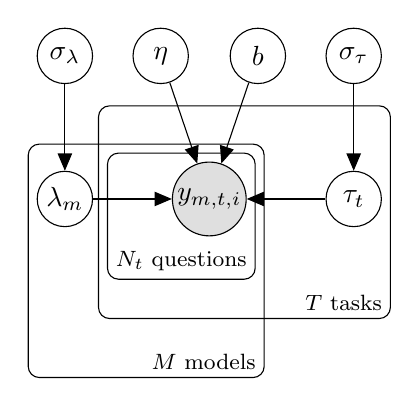
\begin{tikzpicture}
          % nodes
          \node[obs] (obs) {$y_{m,t, i}$};%

          \node[latent, right=of obs, xshift=0.0cm, yshift=-0.0cm] (task_difficulty) {\(\tau_{t}\)}; %

          \node[latent, left=of obs, xshift=0.0cm, yshift=0cm] (model_performance_across_task) {\( \lambda_{m}\)}; 


           \node[latent, above=of task_difficulty, yshift=0.1cm]  (task_difficulty_std) {$\sigma_\tau$ }; 

           \node[latent, above=of model_performance_across_task, yshift=0.0cm, yshift=0.1cm]  (model_performance_across_task_std) {$\sigma_\lambda$ }; 

           
          \node[latent, right=of model_performance_across_task_std, xshift=-0.5cm] (mass) {$\eta$}; 
          
          \node[latent, left=of task_difficulty_std, xshift=0.5cm] (bias) {$b$}; 
          
          % plates
          \coordinate (dummy_bottom) at ([yshift=-1.3cm] obs.south);
          \coordinate (dummy_top) at ([yshift=0.6cm] obs.north);
          \plate [inner sep=0.1cm] {platequestion} {(obs)
          } {$N_t$ questions}; 
          
          \plate [inner sep=0.1cm] {platetask} {
               (platequestion)  (task_difficulty) (dummy_top) % (acc)
          } {$T$ tasks}; 
          
          \plate [inner sep=0.1cm ] {platemodel} {
           (obs) (model_performance_across_task) (dummy_bottom) (platequestion)
          } {$M$ models}; 
          
          % edges
          \edge {task_difficulty, model_performance_across_task, bias, mass} {obs}
          \edge {task_difficulty_std} {task_difficulty}
          \edge {model_performance_across_task_std} {model_performance_across_task}
       
   \end{tikzpicture} 
    }
    \vspace{0.4em}
    \scriptsize Task-based model.
  \end{minipage}\hfill\pause
  \begin{minipage}[t]{0.32\textwidth}
    \centering
    \resizebox{\linewidth}{!}{%
      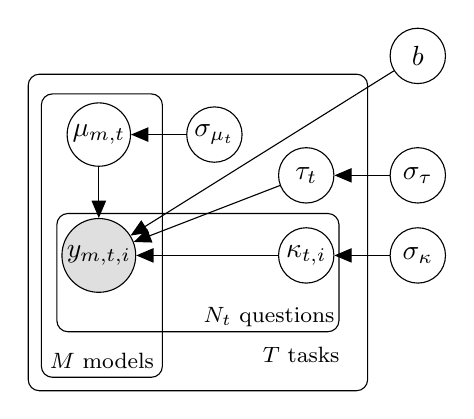
\begin{tikzpicture}
          % nodes
       
          %R
          \node[obs] (acc) {$y_{m,t, i}$};%
          %C
          \node[latent, right=of acc, xshift=0.8cm] (question_difficulty) { $\kappa_{t, i}$ };   
       
          %S
          \node[latent, above=of question_difficulty, xshift=0.0cm, yshift=-0.7cm] (task_difficulty) {\(\tau_{t}\)}; %
       
          \node[latent, above=of acc, xshift=0.0cm, yshift=-0.35cm] (model_performance_specific_task) {\( \mu_{m,t}\)}; 
          \node[latent, right=of model_performance_specific_task,xshift=-0.3cm]  (model_performance_specific_task_std) {\(\sigma_{\mu_t}\)}; %
           
          %global
          \node[latent, right=of question_difficulty, xshift=-0.3cm]  (question_difficulty_std) {$\sigma_\kappa$}; 
          \node[latent, right=of task_difficulty, xshift=-0.3cm]  (task_difficulty_std) {$\sigma_\tau$ }; 
          % Move beta to the global latents
          \node[latent, above=of task_difficulty_std, yshift=-0.2cm] (bias) {$b$}; 
                 
          
          % plates
          % \coordinate (dummy_bottom) at ([xshift=-0.9, yshift=-0.58cm] acc.south);
          \coordinate (dummy_temp) at ([yshift=-0.58cm] acc.south);
          \coordinate (dummy_bottom) at ([xshift=0.7cm] dummy_temp);
          \plate [inner sep=0.10cm ] {platemodel} {(acc) (model_performance_specific_task) (dummy_bottom)} {$M$ models}; 
          \plate [inner sep=0.05cm] {platequestion} {(acc)(question_difficulty)} {$N_t$ questions}; 
          \plate [inner sep=0.35cm] {platetask} {(platequestion)(task_difficulty)(model_performance_specific_task)(model_performance_specific_task_std)} {$T$ tasks}; 
       
          % edges
          \edge {bias, task_difficulty, question_difficulty, model_performance_specific_task} {acc}
          \edge {question_difficulty_std} {question_difficulty}
          \edge {task_difficulty_std} {task_difficulty}
          \edge {model_performance_specific_task_std} {model_performance_specific_task}
       
       \end{tikzpicture} 
    }
    \vspace{0.4em}
    \scriptsize Question-task difficulty model.
  \end{minipage}\hfill
  \pause
  \begin{minipage}[t]{0.32\textwidth}
    \centering
    \resizebox{\linewidth}{!}{%
     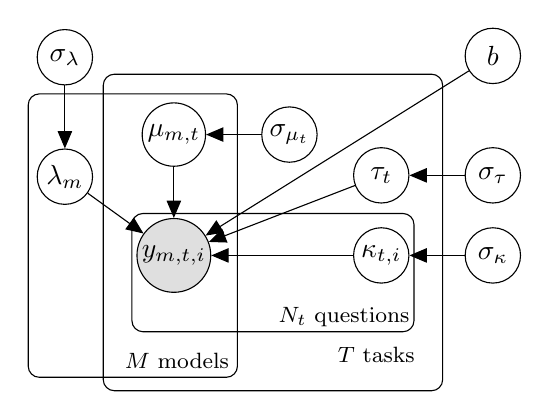
\begin{tikzpicture}
      % nodes

      %R
      \node[obs] (acc) {$y_{m,t, i}$};%
      %C
      \node[latent, right=of acc, xshift=0.8cm] (question_difficulty) { $\kappa_{t, i}$ };   

      %S
      \node[latent, above=of question_difficulty, xshift=0.0cm, yshift=-0.7cm] (task_difficulty) {\(\tau_{t}\)}; %

      \node[latent, above=of acc, xshift=0.0cm, yshift=-0.35cm] (model_performance_specific_task) {\( \mu_{m,t}\)}; 

      \node[latent, left=of acc, xshift=0.45cm, yshift=1.0cm] (model_performance_across_task) {\( \lambda_{m}\)}; 
      
      \node[latent, right=of model_performance_specific_task,xshift=-0.3cm]  (model_performance_specific_task_std) {\(\sigma_{\mu_t}\)}; %
       
      %global
      \node[latent, right=of question_difficulty, xshift=-0.3cm]  (question_difficulty_std) {$\sigma_\kappa$}; 
      \node[latent, right=of task_difficulty,xshift=-0.3cm]  (task_difficulty_std) {$\sigma_\tau$ }; 
      \node[latent, above=of model_performance_across_task, yshift=-0.2cm]  (model_performance_across_task_std) {$\sigma_\lambda$ }; 
      
      % Move beta to the global latents
      \node[latent, above=of task_difficulty_std, yshift=-0.2cm] (bias) {$b$}; 
             
      
      % plates
      % \coordinate (dummy_bottom) at ([yshift=-0.6cm] acc.south);
      \coordinate (dummy_temp) at ([yshift=-0.58cm] acc.south);
      \coordinate (dummy_bottom) at ([xshift=0.7cm] dummy_temp);
      \plate [inner sep=0.10cm ] {platemodel} {(acc) (model_performance_specific_task)  (model_performance_across_task)(dummy_bottom)} {$M$ models}; 
      \plate [inner sep=0.05cm] {platequestion} {(acc)(question_difficulty)} {$N_t$ questions}; 
      \plate [inner sep=0.35cm] {platetask} {(platequestion)(task_difficulty)(model_performance_specific_task)(model_performance_specific_task_std)} {$T$ tasks}; 

      % edges
      \edge {bias, task_difficulty, question_difficulty, model_performance_specific_task, model_performance_across_task} {acc}
      \edge {question_difficulty_std} {question_difficulty}
      \edge {task_difficulty_std} {task_difficulty}
      \edge {model_performance_specific_task_std} {model_performance_specific_task}
      \edge {model_performance_across_task_std} {model_performance_across_task}

   \end{tikzpicture}
    }
    \vspace{0.4em}
    \scriptsize + Across-task performance latent variable.
  \end{minipage}
  \par\vspace{0.8em}\small Graphical models of the proposed hierarchical models. \alert{Way too complicated!}
  
\end{frame}

\begin{frame}{Bayesian Evals for Interpretability}
  \begin{figure}
  \includegraphics[width=\textwidth, height=0.8\textheight, keepaspectratio]{img/bayes_evals/pretrained2.png}
  \end{figure}
  \pause 
  So just use Beta-Binomial!
\end{frame}




\begin{frame}{Future Directions}
  \begin{itemize}[<+->]
    \item If we make our latent variables for `model performance' and `benchmark difficulty' multivariate and sparse, maybe we can interpret their dimensions as different measures of model capability?
    \begin{itemize}
      \item E.g. one dimension is `physics knowledge', another is `reasoning ability' etc.
    \end{itemize}
    \item The results for this were interesting, but not as straightforwardly interpretable as we hoped.
    \item Perhaps these techniques could be used more successfully for predicting eval performance based on the mix of pretraining data?
    \item Or predicting the effectiveness of post-training on downstream evals?
  \end{itemize}
\end{frame}

\begin{frame}{Thank You}
  \begin{itemize}[<+->]
    \item Any questions?
  \end{itemize}
\end{frame}


\begin{frame}[allowframebreaks]{References}
  \nocite{*}
  \printbibliography
\end{frame}


\begin{frame}{IID Questions Setting: Prior Mismatch}
  Use $\theta \sim \text{Uniform}[0, 1]$ as the prior, but $\theta \sim \text{Beta}(100, 20)$ as the true data distribution. ($\mathbb{E}[\theta] = 0.83$ and $\text{Var}(\theta) = 0.034^2$.)
  \begin{figure}
      \includegraphics[width=\textwidth, height=0.75\textheight, keepaspectratio]{img/bayes_evals/fig/exp4-1_beta-100-20_mismatch.pdf}
      % \caption{Simulation results comparing Coverage and Width for different $N$.}
  \end{figure}
\end{frame}

\begin{frame}{Bayesian Evals for Interpretability}
  \begin{itemize}[<+->]
    \item Given eval questions and reponses, use an SAE-like model to enforce sparsity on features across the latent dimensions of `model performance' and `benchmark difficulty' vectors.
  \end{itemize}
  \vspace{-0.2cm}
  \pause
  \begin{figure}
    \includegraphics[width=\textwidth, height=0.77\textheight, keepaspectratio]{img/bayes_evals/fig/task_based_capabilities_IRT_capabilities_3.pdf}
  \end{figure}
\end{frame}


\begin{frame}{Clustered Questions Setting: Bayesian Implementation}
  \begin{figure}
    \includegraphics[width=\textwidth, height=0.8\textheight, keepaspectratio]{img/bayes_evals/bayes_evals_code3.png}
  \end{figure}
\end{frame}

\end{document}"
  % latex -jobname "handout-01" "\def\uselecture{01}\PassOptionsToClass{handout}{beamer}\documentclass[aspectratio=169]{beamer}
% \documentclass[aspectratio=169, handout]{beamer}

\usetheme{Madrid}
\usecolortheme{beaver}

\usepackage{graphicx}
\usepackage{amsmath}
\usepackage{amssymb}
\usepackage{amsthm}
\usepackage{mathrsfs}
\usepackage{hyperref}

\usepackage{tikz}
\usetikzlibrary{bayesnet}
\usetikzlibrary{arrows}


% \usepackage{graphicx}
% \usepackage{booktabs}
% \usepackage{pgfplots}
% \pgfplotsset{compat=1.14}
% \usepackage{anyfontsize}
% % \usepackage{minted}
% \usepackage[cache=false]{minted} 
% \setminted[python]{
%     linenos,
%     % bgcolor=LightGray,
%     % breaklines,
%     fontsize=\scriptsize,
%     % xleftmargin=1.1em,
%     numbersep=4pt
% }

% \usepackage{tcolorbox}

% \newtcolorbox[auto counter]{pbox}[2][]{
%   colback=white,
%   title=#2,
%   #1,
%   fonttitle= \large, %\sffamily,
%   % fontupper=\sffamily,
%   boxrule=0.5pt, 
%   arc=2pt,
%   top=1pt, 
%   bottom=1pt,
%   before={\vspace{2pt}}, 
%   after={\vspace{2pt}} 
%   % colframe=..,
%   % coltitle=..,
%   % colbacktitle=..,
%   % toptitle=0.05cm,
%   % bottomtitle=0.125cm
% }

% \usepackage{fancyvrb}


\setbeamertemplate{caption}{%
  \raggedright
  \insertcaption\par
}

\usepackage[style=authoryear, autocite=footnote, backend=biber]{biblatex}
\addbibresource{refs.bib}

\title[Cohere Research Talk]{Cohere Research Talk: Massively Parallel Inference \& Bayesian Evals}
\author{Sam Bowyer}
\date{November 2025}

\begin{document}

\begin{frame}
  \titlepage
\end{frame}

\begin{frame}{Outline}
  \tableofcontents
\end{frame}

% --- Part 1: Overview ---
\section{About Me}

\begin{frame}{About Me}
  \begin{itemize}[<+->] 
    \item Fourth (final) year PhD student at Bristol's Compass CDT (Computational Statistics and Data Science).
    \item Based in the School of Maths, but supervised by Laurence Aitchison (CS/Engineering Maths), Mengyue Yang (Engineering Maths), and Song Liu (Maths).
    \item Currently working on discrete diffusion models (training an `auxilliary' model with VI to suggest the order in which to decode tokens).
    % \item Also worked on RL and LoRA finetuning.
    \item Two projects I'll be talking about today: Alan (massively parallel probabilistic programming) \& Bayesian Evals.
  \end{itemize}
\end{frame}


% --- Part 2: Alan, Massively Parallel Inference ---
\section{Alan: Massively Parallel Probabilistic Programming}


\begin{frame}{Alan: A Massively Parallel Probabilistic Programming Language}
  \begin{figure}
    \centering
    \includegraphics[height=0.25\textheight]{img/laurence.png}
    \includegraphics[height=0.25\textheight]{img/thomas.png}
    \includegraphics[height=0.25\textheight]{img/sam.png}
    \caption{Work done with Laurence Aitchison and Thomas Heap over the first two years of my PhD.}
  \end{figure}
  \pause
  \begin{itemize}[<+->]
    % \item Work with Laurence Aitchison and Thomas Heap over the first two years of my PhD.
    \item Dual goals:
      \begin{itemize}
        \item Develop `massively parallel' Bayesian inference algorithms: fast, accurate, and scalable; desinged for GPU acceleration.
        \item Implement these algorithms in a probabilistic programming language in pytorch (\texttt{alan}), allowing users to specify general probabilistic models.
      \end{itemize}
  \end{itemize}
\end{frame}


\begin{frame}{Regular Bayesian Inference}
  \begin{itemize}[<+->]
    \item \textbf{Bayesian inference}: Prior $P(z)$ and likelihood $P(x|z)$ for latent variables $z$ and data $x$.
      $$P(z|x) = \frac{P(x|z)P(z)}{\int_\mathcal{Z} P(x,z') dz'}$$
    \item \textbf{Importance sampling}: 
      \begin{enumerate}
        \item Sample $K$ latent variables from a proposal distribution $Q$ (usually IID):
          $$z = (z^1, \ldots, z^K) \sim Q(z).$$ 
        \item Compute importance weights: 
          $$r_k(z) = \frac{P(x , z^k)}{Q(z^k)}.$$ 
        \item Approximate the normalising constant using the `global' estimator: 
          $$\mathcal{P}_\text{global}(z) = \frac{1}{K} \sum_{k=1}^K r_k(z) \quad \text{such that } \quad \mathbb{E}_{z \sim Q}[\mathcal{P}_\text{global}(z)] = P(x).$$ 
      \end{enumerate}
  \end{itemize}
\end{frame}

\begin{frame}{Limitations of Importance Sampling (IS)}
  \begin{itemize}[<+->]
    \item Global IS scales poorly with the number of latent variables, $n$.
    \begin{itemize}
      \item $z^k = (z_1^k, \ldots, z_n^k) \in \mathcal{Z}$.
      % \item E.g. $n$ is the dimension of $z$ if all latent variables are scalar.
    \end{itemize} 
    \item Chatterjee \& Diaconis (2018) show that as $n$ increases, the number of samples, $K$, must increase with $O(e^{D_{\text{KL}}(P(z|x) || Q(z))}) \approx O(e^n)$. (This is a lot!)
    \item Solution: \textbf{Massively Parallel Importance Sampling (MP-IS)}
      \begin{itemize}
        \item Reason about all $K^n$ possible joint samples at once.
      \end{itemize}
  \end{itemize}
\end{frame}


\begin{frame}{Massively Parallel Importance Sampling (MP-IS)}
  \begin{minipage}{0.55\textwidth}
    \begin{figure}
      \includegraphics[width=\textwidth]{img/alan/MPIS.pdf}
    \end{figure}
  \end{minipage}
  \begin{minipage}{0.43\textwidth}
    \begin{itemize}[<+->]
      \item Suppose each latent sample $z^k = (z_1^k, \ldots, z_n^k) \sim Q(z)$ is comprised of $n$ variables.
      \item We can construct $K^n$ different samples from the full joint space 
      $$(z_1^{k_1}, \ldots, z_n^{k_n}) \in \mathcal{Z}$$
      where $\mathbf{k} = (k_1, \ldots, k_n) \in [K]^n$ is the indexing vector for each latent variable.
    \end{itemize}
  \end{minipage}
\end{frame}

\begin{frame}{Massively Parallel Importance Sampling (MP-IS)}
  \begin{minipage}{0.55\textwidth}
    \begin{figure}
      \includegraphics[width=\textwidth]{img/alan/MPIS.pdf}
    \end{figure}
  \end{minipage}
  \begin{minipage}{0.43\textwidth}
    \begin{itemize}[<+->]
      \item Rather than using the global IS estimator
      $$\mathcal{P}_\text{global}(z) = \frac{1}{K} \sum_{k=1}^K \frac{P(x, z^k)}{Q(z^k)}.$$
      \item ...we can use the MP-IS estimator
      $$\mathcal{P}_\text{MP}(z) = \frac{1}{K^n} \sum_{\mathbf{k}\in [K]^n} \frac{P(x, z^\mathbf{k})}{Q_\text{MP}(z^\mathbf{k}, \mathbf{k})}.$$
      (Which is still unbiased.)
    \end{itemize}
  \end{minipage}
\end{frame}

% \begin{frame}{MP-IS: Some Complications...}
%   $$\mathcal{P}_\text{MP}(z) = \frac{1}{K^n} \sum_{\mathbf{k}\in [K]^n} \frac{P(x, z^\mathbf{k})}{Q_\text{MP}(z^\mathbf{k}, \mathbf{k})}.$$
%   \begin{itemize}[<+->]
%     \item We have to be careful about how we define $Q_\text{MP}$ over the space of all $K^n$ joint samples.
%     \item We can use a hierarchical model:
%       $$Q_\text{MP}(z, \mathbf{k}) = \prod_{i=1}^n Q_\text{MP}(z_i^{k_i} | z_j \text{ for } j \in \text{qa}(i)),$$
%       where $\text{qa}(i)$ is the set of indices of parents of $z_i$ in the proposal model.
%     \item If variable $z_i$ has a parent samples $z_j = (z_j^1, \ldots, z_j^K) \sim Q(z_j)$, then we can sample $z_i^{k_i}$ from $Q(z_i^{k_i} | z_j^{\pi(k_i)})$ for a (uniformly) random permutation $\pi$ of $[K]$.  \end{itemize}
% \end{frame}

\begin{frame}{MP-IS: Some Complications...}
  $$\mathcal{P}_\text{MP}(z) = \frac{1}{K^n} \sum_{\mathbf{k}\in [K]^n} \frac{P(x, z^\mathbf{k})}{Q_\text{MP}(z^\mathbf{k}, \mathbf{k})} = \frac{1}{K^n} \sum_{\mathbf{k}\in [K]^n} r_\mathbf{k}(z).$$

  \begin{itemize}[<+->]
    \item We have to be careful about how we define $Q_\text{MP}$ over the space of all $K^n$ joint samples.
    \item Also, at first glance, this thing doesn't look all that nice to compute...
    \item But we can exploit the conditional independencies in the model to render it tractable.
  \end{itemize}

\end{frame}


\begin{frame}{MP-IS: Some Complications...}

  \begin{figure}
    \includegraphics[width=0.6\textwidth]{img/alan/toy_model.drawio.pdf}
  \end{figure}

  \begin{itemize}[<+->]
    \item E.g. with the model from before with $n=3$, $P(x, z) =  P(z_1) P(z_2 | z_1) P(z_3 | z_2) P(x | z_3)$, we can move the sums inside the product and get a bunch of tensor products:
  \end{itemize}
    \pause
    $$
    % \begin{aligned}
      \mathcal{P}_\text{MP}(z) = \frac{1}{K^3} \sum_{k_1 \in [K]} \sum_{k_2 \in [K]} \sum_{k_3 \in [K]} \frac{P(z_1^{k_1}) P(z_2^{k_2} | z_1^{k_1}) P(z_3^{k_3} | z_2^{k_2}) P(x | z_3^{k_3})}{Q(z_1^{k_1}) Q(z_2^{k_2}) Q(z_3^{k_3})}
      % = \frac{1}{K^3} \sum_{k_1 \in [K]} \sum_{k_2 \in [K]} \sum_{k_3 \in [K]} r_{k_1,k_2,k_3}(z)
    $$
    \pause
    $$
      = \frac{1}{K^3} \sum_{k_1 \in [K]} \underbrace{\frac{P(z_1^{k_1})}{Q(z_1^{k_1})}}_{\text{Vector of size } K} 
      \sum_{k_2 \in [K]} \underbrace{\frac{P(z_2^{k_2} | z_1^{k_1})}{Q(z_2^{k_2})}}_{\text{Matrix of size } K \times K}
      \sum_{k_3 \in [K]} \underbrace{\frac{P(z_3^{k_3} | z_2^{k_2})}{Q(z_3^{k_3})}}_{\text{Matrix of size } K \times K}
      \underbrace{P(x | z_3^{k_3})}_{\text{Vector of size } K}
    % \end{aligned}
    $$
    % \item This can be computed efficiently on a GPU using tensor operations.
  % \end{itemize}
\end{frame}


\begin{frame}{Can we hide these complications from the user?}
  \begin{itemize}[<+->]
    \item Yes! We do this with \texttt{alan}.
    \item User specifies the model with P and Q as pytorch modules, and we handle the massively parallel inference for them.
  \end{itemize}
\end{frame}

\begin{frame}{Alan: A Probabilistic Programming Language}

  \begin{minipage}{0.7\textwidth}
    \begin{figure}
      \centering
      \includegraphics[width=0.9\textwidth]{img/alan/movielens_code_1.png}
    \end{figure}
  \end{minipage}
  \begin{minipage}{0.25\textwidth}
    % \vspace{-1cm}
    \begin{figure}[t]
      \centering
      \resizebox{0.8\textwidth}{!}{%
        \tikz{
          % nodes
           \node[obs] (rating) {\(\mathrm{Rating}_{mn}\)};%
           \node[latent,above=of rating] (peruser) {\(\mathbf{z}_m\)}; %
           \node[latent, above=of peruser, xshift=-1cm] (psi) {\(\boldsymbol{\psi}\)};
          \node[latent, above=of peruser, xshift=1cm] (mu) {\(\boldsymbol{\mu}\)};
          % plate
           \plate [inner sep=.3cm] {plate2} {(rating)} {\(\mathrm{N}\) Films}; %
           \plate [inner sep=.3cm] {plate1} {(peruser)(plate2)} {\(\mathrm{M}\) Users}; %
          edges
           \edge {psi,mu} {peruser}
           \edge {peruser} {rating}}
           }
    \end{figure}
  \end{minipage}

\end{frame}

\begin{frame}{MP-VI}
  \begin{itemize}[<+->]
    \item Using $\mathcal{P}_\text{MP}(z)$, we can do variational inference (VI) by maximising the ELBO:
      $$
      \log P(x) \geq \mathcal{L}_\text{MP}(\theta) = \mathbb{E}_{z \sim Q_\text{MP}(\theta)}[\log \mathcal{P}_\text{MP}(z)]
      $$
    \item Aitchison (2019) showed that MP-VI is a tighter bound than the global VI objective (IWAE):
      $$
      \log P(x) \geq \mathcal{L}_\text{MP}(\theta) \geq \mathcal{L}_\text{global}(\theta) = \mathbb{E}_{z \sim Q(\theta)}[\log \mathcal{P}_\text{global}(z)]
      $$
  \end{itemize}
  \pause
  \begin{figure}
    \centering
    \includegraphics[width=0.9\textwidth]{img/alan/movielens_code_2.png}
  \end{figure}
\end{frame}

\begin{frame}{MP Algorithms}
  \begin{itemize}[<+->]
    \item We can obtain unbiased posterior moment estimates via autodiff (Bowyer et al. (2024)).
      $$
      m_\text{MP}(z) = \frac{1}{K^n} \sum_{\mathbf{k} \in [K]^n} \frac{r_\mathbf{k}(z)}{\mathcal{P}_\text{MP}(z)}m(z^\mathbf{k})
      $$
    \item We define a modified marginal likelihood estimator with an auxiliary variable $J \in \mathbb{R}$:
      $$
      \mathcal{P}_\text{MP}^\text{exp}(z, J) = \frac{1}{K^n} \sum_{\mathbf{k} \in [K]^n} r_\mathbf{k}(z) \exp(J m(z^\mathbf{k}))
      $$
    \item Then differentiating the log of this with respect to $J$ and setting $J=0$ we get:
      $$
      \frac{\partial}{\partial J}\bigg|_{J=0} \log \mathcal{P}_\text{MP}^\text{exp} (z, J) = \frac{\frac{\partial}{\partial J}\bigg|_{J=0} \mathcal{P}_\text{MP}^\text{exp} (z, J)}{\mathcal{P}_\text{MP}^\text{exp} (z, 0)} = m_\text{MP}(z)
      $$
    \item By similar arguments: $J \in \mathbb{R}^K$ gives us marginal importance weights; $J \in \mathbb{R}^{K^{1+|pa(i)|}}$ gives us importance samples for $z_i$, given its parents $pa(i)$.
  \end{itemize}
  \vspace{0.1cm}
\end{frame}

\begin{frame}{QEM: An Adaptive Importance Sampling Algorithm}
  \begin{minipage}{0.4\textwidth}
    \textbf{QEM} (Heap et al. (2025))
    \begin{enumerate}
      \item Start with an initial approximate posterior $Q_0$.
      \item Compute posterior moment estimates $m_\text{MP}(z)$ using MP-IS.
      \item Update the approximate posterior $Q_{t+1}$ using the moment estimates.
    \end{enumerate}    
  
    Can be seen as an EM-like algorithm for adaptive imortance sampling.
  \end{minipage}
  \begin{minipage}{0.59\textwidth}
    \begin{figure}
      \centering
      \includegraphics[width=0.95\textwidth]{img/alan/QEM_results.pdf}
    \end{figure}
  \end{minipage}
\end{frame}

\begin{frame}{Conclusions}
  \begin{itemize}[<+->]
    \item This project was a great (if, at times, complicated) way to learn about Bayesian inference and numerical and probabilistic programming.
    \item The results were pretty promising, but but there are some drawbacks to massively parallel methods:
    \begin{itemize}
      \item The algorithms are complex to implement (hence wrapping them in a PPL).
      \item Not all models have lots of conditional independencies to exploit.
      \item Although it's slower and harder to tune, HMC is often hard to beat in terms of quality of inference.
    \end{itemize}
  \end{itemize}
\end{frame}

% --- Part 3: Bayesian Evals, Uncertainty Quantification for LLM Evals ---
\section{Bayesian Evals: Uncertainty Quantification for LLM Evals}

\begin{frame}{Bayesian Evals: Uncertainty Quantification for LLM Evals}
  \begin{figure}
    \centering
    \includegraphics[height=0.25\textheight]{img/laurence.png}
    \includegraphics[height=0.25\textheight]{img/desi.jpg}
    \includegraphics[height=0.25\textheight]{img/sam.png}
    \caption{Work done with Laurence Aitchison and Desi R. Ivanova.}
  \end{figure}
  \begin{itemize}[<+->]
    \item Two directions:
      \begin{itemize}
        \item Improved UQ for evals with Bayesian methods.
        \item Interpretability of evals with Bayesian hierarchical modelling and SAE-like approaches.
      \end{itemize}
    \item The former direction led to an ICML spotlight position paper: \emph{`Position: Don't Use the CLT in LLM Evals With Fewer Than a Few Hundred Datapoints'}.
    \item The latter fell by the wayside, but is something I'd like to come back to at some point.
  \end{itemize}
\end{frame}

% --- Slide 2: Motivation ---
\begin{frame}{Motivation}
  \begin{block}{Central Limit Theorem (CLT)}
    If $X_1, \dots, X_N$ are IID r.v.s with mean $\mu \in \mathbb{R}$ and finite variance $\sigma^2$, then 
    $$
      \sqrt{N} (\hat{\mu} - \mu) \xrightarrow{d} \mathcal{N}( 0, \sigma^2 ) \; \text{as } N \rightarrow \infty,
    $$
    where $\hat{\mu} = \frac{1}{N}\sum_{i=1}^N X_i$ is the sample mean.
  \end{block}
  \pause
  \begin{itemize}[<+->]
      % \item Error bars are important for interpreting evals.
      \item The CLT-based confidence interval is:
      $$
        \text{CI}_{1-\alpha}(\mu) = \hat{\mu} \pm z_{\alpha/2} \text{SE}(\hat{\mu})
      $$
      where $z_{\alpha/2}$ is the $100(1-\alpha/2)$-th percentile of $\mathcal{N}(0, 1)$ and $\text{SE}(\hat{\mu}) = \sqrt{\frac{\hat{\sigma}^2}{N}}$ is the standard error of the sample mean.
      \item In the case of binary data $X_i \in \{0, 1\}$, this becomes:
      $$
        \text{CI}_{1-\alpha}(\theta) = \bar{X} \pm z_{\alpha/2} \sqrt{\bar{X}(1-\bar{X})/N}.
      $$
  \end{itemize}
  
\end{frame}

\begin{frame}{Real-World Failures of the CLT}
  \begin{itemize}[<+->]
    \item If $N$ is too small, CLT-based error bars can collapse to \alert{zero-width} or \alert{extend past $[0,1]$}.
    \item Smaller, more intricate, and expensive LLM benchmarks are becoming increasingly common, so we need to find alternatives for the few-data regime.
  \end{itemize}
  % \vspace{0.5cm}
  \begin{minipage}{0.45\textwidth}
    \centering
    \begin{figure}
      \includegraphics[height=4.2cm, keepaspectratio]{img/bayes_evals/pngs/real_data_matharena_aime_II_subset.png}
      \caption{Math Arena's AIME II 2025 Benchmark (N=15). Various 95\% interval types shown.}
    \end{figure}
  \end{minipage}
  \begin{minipage}{0.45\textwidth}
    \centering
    \begin{figure}
        \includegraphics[height=4.2cm, keepaspectratio]{img/bayes_evals/langchain_clt.png}
        \caption{Langchain Typewriter Tool Use Benchmark (N=20). CLT-based 95\% intervals only.}
    \end{figure}
  \end{minipage}
\end{frame}

% --- Slide 3: Bayesian Alternative -- Beta-Bernoulli Model ---
\begin{frame}{Bayesian Alternative: Beta-Binomial Model}
  \begin{itemize}[<+->]
    \item Treat the data as IID Bernoulli with a \alert{uniform prior} on the parameter $\theta$.
    $$
      \begin{aligned}
      \theta &\sim \text{Beta}(1, 1) = \text{Uniform}[0, 1] \\
      y_i &\sim \text{Bernoulli}(\theta) \; \text{for } i=1,\dots N 
      \end{aligned}
    $$
    \item Say $y_i$ is correct if $y_i = 1$ and incorrect if $y_i = 0$. %(Think of $\theta$ as the probability of correctness.)  
    \item Obtain quantile-based Bayesian \alert{credible intervals} for $\theta$ from the closed form posterior.
    $$
      p(\theta | y_{1:N}) = \text{Beta}\left(1+\sum_{i=1}^N y_i, 1 + \sum_{i=1}^N (1-y_i)\right)
    $$

  \end{itemize}
  
\pause
\begin{figure}
  \centering
  \includegraphics[width=0.8\textwidth]{img/bayes_evals/bayes_evals_code1.png}
\end{figure}


% \begin{pbox}[label={ex:bayes_simple}]{Beta-Bernoulli Bayesian Credible Interval}
%   \begin{minted}[fontsize=\scriptsize,breaklines]{python}
%  y is a length N binary "eval" vector
% S, N = y.sum(), len(y)  total successes & questions

% # Bayesian Credible interval
% posterior = scipy.stats.beta(1 + sum(y), 1 + N - sum(y))
% bayes_ci  = posterior.interval(confidence=0.95)
%   \end{minted}
% \end{pbox}

\end{frame}

% --- Slide 4: Frequentist Alternatives ---
\begin{frame}{Frequentist Alternatives}
  % \vspace{1cm}
  \begin{itemize}[<+->]
      \item \alert{Wilson score interval}: Based on normal approximation to the binomial distribution.
        \pause
        $$ \text{CI}_{1-\alpha, \text{Wilson}}(\theta) = \frac{\hat{\theta} + \frac{z_{\alpha/2}^2}{2N}}{1 + \frac{z_{\alpha/2}^2}{N}} \pm \frac{\frac{z_{\alpha/2}}{2N}}{1 + \frac{z_{\alpha/2}^2}{N}}\sqrt{4N\hat{\theta}(1 - \hat{\theta}) + z_{\alpha/2}^2} $$
        \pause
      \item \alert{Clopper-Pearson `exact' interval}: A `worst-case' approach; very conservative method guaranteed to never under-cover.
      $\text{CI}_{1-\alpha, \text{CP}}(\theta) = [\theta_\text{lower}, \theta_\text{upper}]$, 
        \pause
        $$ \theta_\text{lower} = B\left(\frac{\alpha}{2}, \sum_{i=1}^N y_i, 1+\sum_{i=1}^N(1-y_i)\right) \; \text{and} \; \theta_\text{upper} = B\left(1-\frac{\alpha}{2}, 1+ \sum_{i=1}^N y_i, \sum_{i=1}^N(1-y_i)\right) $$
        where $B(\alpha, a, b)$ is the $\alpha$-th quantile of the Beta$(a, b)$ distribution.
  \end{itemize}
  
  \pause
  % \vspace{1cm}
  % Implementation using \texttt{scipy}:
%   \begin{verbatim}
% # y is a length N binary "eval" vector
% S, N = y.sum(), len(y) # total successes & questions
% result = scipy.stats.binomtest(k=S, n=N)

% # 95% Wilson score interval and Clopper-Pearson exact interval
% wilson_ci = result.proportion_ci("wilson", 0.95)
% cp_ci = result.proportion_ci("exact", 0.95)
%   \end{verbatim}
\begin{figure}
  \centering
  \includegraphics[width=0.8\textwidth]{img/bayes_evals/bayes_evals_code2.png}
\end{figure}
\end{frame}

% --- Slide 5: Interval Comparison Simulations ---
\begin{frame}{Interval Comparison Simulations}
  \vspace{1cm}
  We use synthetic eval data so that we \alert{know} the true parameter $\theta$.
  
  \begin{itemize}[<+->]
      \item Draw $\theta \sim \text{Uniform}[0, 1]$.
      \item Draw $N \in \{3,10,30,100\}$ IID Bernoulli datapoints with parameter $\theta$.
      \item Construct intervals with various methods for various $1-\alpha$ confidence levels.
      \item Repeat many times and calculate the true coverage and average width of the intervals.
      \begin{itemize}
        \item Coverage: What proportion of the time does a $1-\alpha$ confidence-level interval \alert{actually contain} the true parameter? (A frequentist metric, really.)
        \item Ideally, $\text{coverage} = 1-\alpha$.
      \end{itemize}
  \end{itemize}
\end{frame}

% --- Slide 6: IID Questions Setting ---
\begin{frame}{IID Questions Setting: Results}
  \begin{figure}
      \includegraphics[width=\textwidth, height=0.8\textheight, keepaspectratio]{img/bayes_evals/fig/exp4-1_top_row_only.pdf}
      % \caption{Simulation results comparing Coverage and Width for different $N$.}
  \end{figure}
\end{frame}

\begin{frame}{IID Questions Setting: Results}
  \begin{figure}
      \includegraphics[width=\textwidth, height=0.8\textheight, keepaspectratio]{img/bayes_evals/fig/exp4-1_inkscape.pdf}
      % \caption{Simulation results comparing Coverage and Width for different $N$.}
  \end{figure}
\end{frame}

% --- Slide 7: Other Eval Settings ---
\begin{frame}{Other Eval Settings}
  \begin{itemize}[<+->]
      \item \textbf{Clustered Questions}
      \begin{itemize}
          \item Instead of $N$ IID questions, we have $T$ tasks, each with $N_t$ IID questions.
      \end{itemize}
      
      \item \textbf{Comparisons Between Two Models, $\theta_A$ and $\theta_B$}
      \begin{itemize}
          \item Independent Comparisons (using $N_A, N_B, \bar{y}_A, \bar{y}_B$ only).
          \item Paired Comparisons (using $N_A = N_B, \{y_{A;i}\}_{i=1}^N, \{y_{B;i}\}_{i=1}^N$).
          % \item Hypothesis testing $H_0: \theta_A = \theta_B$ vs $H_1: \theta_A > \theta_B$.
          \item With Bayes you can calculate $\mathbb{P}(\theta_A > \theta_B | y_A, y_B)$.
      \end{itemize}
      
      \item \textbf{Metrics that aren't simple averages of binary results} (e.g. F1 score).
      
      \item \textbf{Prior Mismatch} (i.e. what if the uniform prior is incorrect, $\theta \nsim \text{Uniform}[0, 1]$?).
  \end{itemize}
\end{frame}


% --- Slide 8: Clustered Questions Setting ---
\begin{frame}{Clustered Questions Setting: Frequentist Approach}
  \begin{itemize}[<+->]
    \item Instead of $N$ IID questions, we have $T$ tasks, each with $N_t$ IID questions.
    \item Some tasks are easier than others.% (e.g. each task asks $N_t$ questions about a single piece of input text, with texts varying in difficulty).
    \item Frequentist approach (Miller, 2024):
    $$
    \text{CI}_{1-\alpha}(\theta) = \bar{X} \pm z_{\alpha/2} \text{SE}_\text{Clustered}
    $$
    $$
    \text{SE}_\text{Clustered} = \sqrt{\text{SE}_\text{CLT}^2 + \frac{1}{N^2}\sum_{t=1}^T \sum_{i=1}^{N_t} \sum_{j \neq i} (y_{i,t} - \bar{y})(y_{j,t} - \bar{y})}
    $$
    % \item An improved standard error, but fundamentally still using the CLT.
  \end{itemize}
\end{frame}


\begin{frame}{Clustered Questions Setting: A Bayesian Approach}
  \begin{itemize}[<+->]
    \item `Dispersion' parameter $d$ controls the range of difficulty across tasks,
    $$d \sim \text{Gamma}(1, 1).$$
    \item $\theta$ is the mean difficulty of the questions across tasks,
    $$
    \theta \sim \text{Beta}(1, 1) = \text{Uniform}[0, 1].
    $$
    \item $\theta_t$ is the difficulty of the questions in task $t$ (we ensure that $\mathbb{E}[\theta_t | \theta] = \theta$),
    $$  
    \theta_t \sim \text{Beta}(d \theta, d (1-\theta)).
    $$
    \item $\text{Var}(\theta_t | \theta) = \frac{\theta (1-\theta)}{d^2 + 1}$.
    \item If $d$ is large, then $\theta_t$ is close to $\theta$ for all tasks.
    \item If $d$ is small, then $\theta_t$ is more variable across tasks.
  \end{itemize}
\end{frame}

\begin{frame}{Clustered Questions Setting: A Bayesian Approach}
  \vspace{-0.5cm}
  $$
    \begin{aligned}
    d &\sim \text{Gamma}(1, 1), \quad 
    \theta \sim \text{Beta}(1, 1), \quad 
    \theta_t &\sim \text{Beta}(d \theta, d (1-\theta)), \quad
    y_{i,t} \sim \text{Bernoulli}(\theta_t)
    \end{aligned}
  $$
  \vspace{-0.5cm}
  \pause
  \begin{itemize}[<+->]
    \item Can we integrate out the per-task difficulty parameters $\theta_t$?
    \item Yes! The number of successes per task is \alert{Beta-Binomial} distributed: 
      $$
        \sum_{i=1}^{N_t} y_{i,t} = Y_t \sim \text{BetaBinomial}(N_t, d \theta, d (1-\theta)).
      $$
    \item Get an \alert{importance-weighted posterior} for $\theta$: draw prior samples $\{(\theta^{(k)}, d^{(k)})\}_{k=1}^K$, then compute weights
      $$
        w^{(k)} = \prod_{t=1}^T p(Y_t | \theta^{(k)}, d^{(k)}).
      $$
    \item Compute quantile-based Bayesian credible intervals for $\theta$.
  \end{itemize}
\end{frame}

\begin{frame}{Clustered Questions Setting: Results}
  \begin{figure}
      \includegraphics[width=\textwidth, height=0.8\textheight, keepaspectratio]{img/bayes_evals/pngs/exp4-2.png}
      % \caption{Simulation results comparing Coverage and Width for different $N$.}
  \end{figure}
\end{frame}


% --- Slide 9: Conclusion ---
\begin{frame}{Conclusion}
  Advice to practitioners:
  
  \begin{itemize}[<+->]
      \item Use \alert{Bayesian Beta-Bernoulli} or \alert{Wilson Score intervals} for IID setting.
      \item Use simple \alert{Bayesian models} for other settings (for flexibility and interpretability).
      \item It's \textbf{easy} (use \texttt{scipy} or \texttt{bayes\_evals}).
      \item It's \textbf{safer} than CLT-based methods.
      \item It's still \textbf{cheap} for large $N$.
  \end{itemize}
  
  \vspace{1cm}

  \pause
  My takeaways from this project:
  \begin{itemize}[<+->]
    \item The project really cemented my understanding of Bayesianism vs Frequentism in practice.
    \item There's a big communication gap between AI researchers and classical statisticians.
    \item UQ for evals is an incredibly rich space.
  \end{itemize}
  % \begin{columns}
  %     \column{0.5\textwidth}
  %     \centering
  %     \textbf{Paper} \\
  %     \href{https://arxiv.org/pdf/2503.01747}{https://arxiv.org/pdf/2503.01747} \\
  %     \vspace{0.5cm}
  %     \includegraphics[width=3cm]{img/bayes_evals/arxiv_qr.png}
      
  %     \column{0.5\textwidth}
  %     \centering
  %     \textbf{\texttt{bayes\_evals} package} \\
  %     \href{https://github.com/sambowyer/bayes_evals}{https://github.com/sambowyer/bayes\_evals} \\
  %     \vspace{0.5cm}
  %     \includegraphics[width=3cm]{img/bayes_evals/github_qr.png}
  % \end{columns}
\end{frame}


\begin{frame}{Bayesian Evals for Interpretability}
  \begin{itemize}[<+->]
    \item Apply hierarchical Bayesian modelling to evals: infer latent variables for \alert{benchmark difficulty} and \alert{model performance}.
  \end{itemize}

  \pause
  
  \begin{minipage}[t]{0.32\textwidth}
    \centering
    \resizebox{\linewidth}{!}{%
      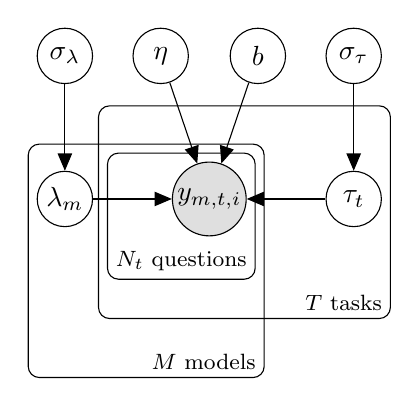
\begin{tikzpicture}
          % nodes
          \node[obs] (obs) {$y_{m,t, i}$};%

          \node[latent, right=of obs, xshift=0.0cm, yshift=-0.0cm] (task_difficulty) {\(\tau_{t}\)}; %

          \node[latent, left=of obs, xshift=0.0cm, yshift=0cm] (model_performance_across_task) {\( \lambda_{m}\)}; 


           \node[latent, above=of task_difficulty, yshift=0.1cm]  (task_difficulty_std) {$\sigma_\tau$ }; 

           \node[latent, above=of model_performance_across_task, yshift=0.0cm, yshift=0.1cm]  (model_performance_across_task_std) {$\sigma_\lambda$ }; 

           
          \node[latent, right=of model_performance_across_task_std, xshift=-0.5cm] (mass) {$\eta$}; 
          
          \node[latent, left=of task_difficulty_std, xshift=0.5cm] (bias) {$b$}; 
          
          % plates
          \coordinate (dummy_bottom) at ([yshift=-1.3cm] obs.south);
          \coordinate (dummy_top) at ([yshift=0.6cm] obs.north);
          \plate [inner sep=0.1cm] {platequestion} {(obs)
          } {$N_t$ questions}; 
          
          \plate [inner sep=0.1cm] {platetask} {
               (platequestion)  (task_difficulty) (dummy_top) % (acc)
          } {$T$ tasks}; 
          
          \plate [inner sep=0.1cm ] {platemodel} {
           (obs) (model_performance_across_task) (dummy_bottom) (platequestion)
          } {$M$ models}; 
          
          % edges
          \edge {task_difficulty, model_performance_across_task, bias, mass} {obs}
          \edge {task_difficulty_std} {task_difficulty}
          \edge {model_performance_across_task_std} {model_performance_across_task}
       
   \end{tikzpicture} 
    }
    \vspace{0.4em}
    \scriptsize Task-based model.
  \end{minipage}\hfill\pause
  \begin{minipage}[t]{0.32\textwidth}
    \centering
    \resizebox{\linewidth}{!}{%
      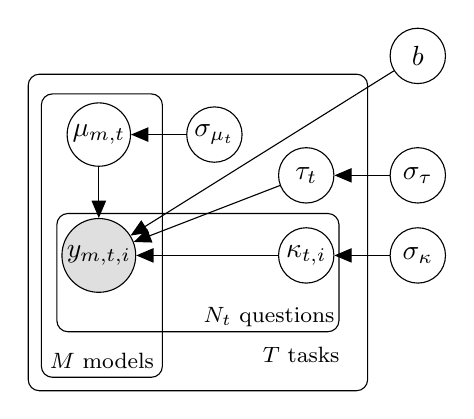
\begin{tikzpicture}
          % nodes
       
          %R
          \node[obs] (acc) {$y_{m,t, i}$};%
          %C
          \node[latent, right=of acc, xshift=0.8cm] (question_difficulty) { $\kappa_{t, i}$ };   
       
          %S
          \node[latent, above=of question_difficulty, xshift=0.0cm, yshift=-0.7cm] (task_difficulty) {\(\tau_{t}\)}; %
       
          \node[latent, above=of acc, xshift=0.0cm, yshift=-0.35cm] (model_performance_specific_task) {\( \mu_{m,t}\)}; 
          \node[latent, right=of model_performance_specific_task,xshift=-0.3cm]  (model_performance_specific_task_std) {\(\sigma_{\mu_t}\)}; %
           
          %global
          \node[latent, right=of question_difficulty, xshift=-0.3cm]  (question_difficulty_std) {$\sigma_\kappa$}; 
          \node[latent, right=of task_difficulty, xshift=-0.3cm]  (task_difficulty_std) {$\sigma_\tau$ }; 
          % Move beta to the global latents
          \node[latent, above=of task_difficulty_std, yshift=-0.2cm] (bias) {$b$}; 
                 
          
          % plates
          % \coordinate (dummy_bottom) at ([xshift=-0.9, yshift=-0.58cm] acc.south);
          \coordinate (dummy_temp) at ([yshift=-0.58cm] acc.south);
          \coordinate (dummy_bottom) at ([xshift=0.7cm] dummy_temp);
          \plate [inner sep=0.10cm ] {platemodel} {(acc) (model_performance_specific_task) (dummy_bottom)} {$M$ models}; 
          \plate [inner sep=0.05cm] {platequestion} {(acc)(question_difficulty)} {$N_t$ questions}; 
          \plate [inner sep=0.35cm] {platetask} {(platequestion)(task_difficulty)(model_performance_specific_task)(model_performance_specific_task_std)} {$T$ tasks}; 
       
          % edges
          \edge {bias, task_difficulty, question_difficulty, model_performance_specific_task} {acc}
          \edge {question_difficulty_std} {question_difficulty}
          \edge {task_difficulty_std} {task_difficulty}
          \edge {model_performance_specific_task_std} {model_performance_specific_task}
       
       \end{tikzpicture} 
    }
    \vspace{0.4em}
    \scriptsize Question-task difficulty model.
  \end{minipage}\hfill
  \pause
  \begin{minipage}[t]{0.32\textwidth}
    \centering
    \resizebox{\linewidth}{!}{%
     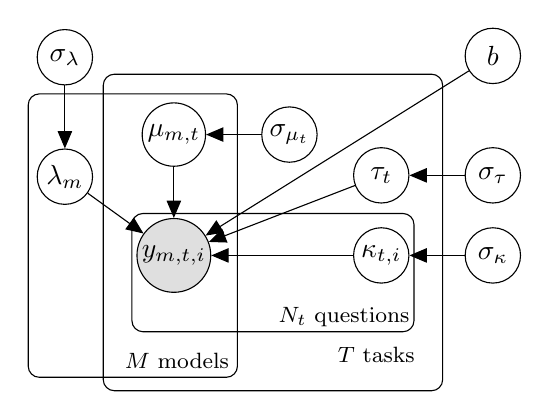
\begin{tikzpicture}
      % nodes

      %R
      \node[obs] (acc) {$y_{m,t, i}$};%
      %C
      \node[latent, right=of acc, xshift=0.8cm] (question_difficulty) { $\kappa_{t, i}$ };   

      %S
      \node[latent, above=of question_difficulty, xshift=0.0cm, yshift=-0.7cm] (task_difficulty) {\(\tau_{t}\)}; %

      \node[latent, above=of acc, xshift=0.0cm, yshift=-0.35cm] (model_performance_specific_task) {\( \mu_{m,t}\)}; 

      \node[latent, left=of acc, xshift=0.45cm, yshift=1.0cm] (model_performance_across_task) {\( \lambda_{m}\)}; 
      
      \node[latent, right=of model_performance_specific_task,xshift=-0.3cm]  (model_performance_specific_task_std) {\(\sigma_{\mu_t}\)}; %
       
      %global
      \node[latent, right=of question_difficulty, xshift=-0.3cm]  (question_difficulty_std) {$\sigma_\kappa$}; 
      \node[latent, right=of task_difficulty,xshift=-0.3cm]  (task_difficulty_std) {$\sigma_\tau$ }; 
      \node[latent, above=of model_performance_across_task, yshift=-0.2cm]  (model_performance_across_task_std) {$\sigma_\lambda$ }; 
      
      % Move beta to the global latents
      \node[latent, above=of task_difficulty_std, yshift=-0.2cm] (bias) {$b$}; 
             
      
      % plates
      % \coordinate (dummy_bottom) at ([yshift=-0.6cm] acc.south);
      \coordinate (dummy_temp) at ([yshift=-0.58cm] acc.south);
      \coordinate (dummy_bottom) at ([xshift=0.7cm] dummy_temp);
      \plate [inner sep=0.10cm ] {platemodel} {(acc) (model_performance_specific_task)  (model_performance_across_task)(dummy_bottom)} {$M$ models}; 
      \plate [inner sep=0.05cm] {platequestion} {(acc)(question_difficulty)} {$N_t$ questions}; 
      \plate [inner sep=0.35cm] {platetask} {(platequestion)(task_difficulty)(model_performance_specific_task)(model_performance_specific_task_std)} {$T$ tasks}; 

      % edges
      \edge {bias, task_difficulty, question_difficulty, model_performance_specific_task, model_performance_across_task} {acc}
      \edge {question_difficulty_std} {question_difficulty}
      \edge {task_difficulty_std} {task_difficulty}
      \edge {model_performance_specific_task_std} {model_performance_specific_task}
      \edge {model_performance_across_task_std} {model_performance_across_task}

   \end{tikzpicture}
    }
    \vspace{0.4em}
    \scriptsize + Across-task performance latent variable.
  \end{minipage}
  \par\vspace{0.8em}\small Graphical models of the proposed hierarchical models. \alert{Way too complicated!}
  
\end{frame}

\begin{frame}{Bayesian Evals for Interpretability}
  \begin{figure}
  \includegraphics[width=\textwidth, height=0.8\textheight, keepaspectratio]{img/bayes_evals/pretrained2.png}
  \end{figure}
  \pause 
  So just use Beta-Binomial!
\end{frame}




\begin{frame}{Future Directions}
  \begin{itemize}[<+->]
    \item If we make our latent variables for `model performance' and `benchmark difficulty' multivariate and sparse, maybe we can interpret their dimensions as different measures of model capability?
    \begin{itemize}
      \item E.g. one dimension is `physics knowledge', another is `reasoning ability' etc.
    \end{itemize}
    \item The results for this were interesting, but not as straightforwardly interpretable as we hoped.
    \item Perhaps these techniques could be used more successfully for predicting eval performance based on the mix of pretraining data?
    \item Or predicting the effectiveness of post-training on downstream evals?
  \end{itemize}
\end{frame}

\begin{frame}{Thank You}
  \begin{itemize}[<+->]
    \item Any questions?
  \end{itemize}
\end{frame}


\begin{frame}[allowframebreaks]{References}
  \nocite{*}
  \printbibliography
\end{frame}


\begin{frame}{IID Questions Setting: Prior Mismatch}
  Use $\theta \sim \text{Uniform}[0, 1]$ as the prior, but $\theta \sim \text{Beta}(100, 20)$ as the true data distribution. ($\mathbb{E}[\theta] = 0.83$ and $\text{Var}(\theta) = 0.034^2$.)
  \begin{figure}
      \includegraphics[width=\textwidth, height=0.75\textheight, keepaspectratio]{img/bayes_evals/fig/exp4-1_beta-100-20_mismatch.pdf}
      % \caption{Simulation results comparing Coverage and Width for different $N$.}
  \end{figure}
\end{frame}

\begin{frame}{Bayesian Evals for Interpretability}
  \begin{itemize}[<+->]
    \item Given eval questions and reponses, use an SAE-like model to enforce sparsity on features across the latent dimensions of `model performance' and `benchmark difficulty' vectors.
  \end{itemize}
  \vspace{-0.2cm}
  \pause
  \begin{figure}
    \includegraphics[width=\textwidth, height=0.77\textheight, keepaspectratio]{img/bayes_evals/fig/task_based_capabilities_IRT_capabilities_3.pdf}
  \end{figure}
\end{frame}


\begin{frame}{Clustered Questions Setting: Bayesian Implementation}
  \begin{figure}
    \includegraphics[width=\textwidth, height=0.8\textheight, keepaspectratio]{img/bayes_evals/bayes_evals_code3.png}
  \end{figure}
\end{frame}

\end{document}"
  \expandafter\includeonlylecture\expandafter{\uselecture}
\else
  % Default lecture to output - comment out to get all lectures
  \includeonlylecture{01} 
\fi

% Uncomment to get title slides for each lecture
% \AtBeginLecture{
%   \subtitle{\insertlecture}
%   \setcounter{framenumber}{0}
%   \begin{frame}
%     \titlepage
%   \end{frame}
% } 

\AtBeginSection[]
{
    \begin{frame}
        \frametitle{Table of Contents}
        \tableofcontents[currentsection]
    \end{frame}
}

\usepackage[style=authoryear-ibid,
            autocite=footnote,
            backend=biber,
           ]{biblatex}

\addbibresource{refs.bib} 

\let\oldfootnote\footnote
\renewcommand{\footnote}{\only<+->\oldfootnote}



%%%%%%%%%%%%%%%%%%%%%%%%%%%%%%%%%%%%%%%%%%%%%%%%%%%%%%%%%%%%%%%%%%%%%%%%%%%%%%
% Start of the slides

\begin{document}

% Available frame options:
%   leftcolor, rightcolor: set the colour of the left or right panel
%   leftimage, rightimage: put a (cropped) image in the left or right panel
%   div: set the location of the divider between left and right panels
%   urlcolor: set the colour of the url

% Other commands available:
%   \logo{X}: choose the logo to display (logo, white logo, or black logo)
%   \urltext{X}: change the url for each slide

% All standard University of Bristol colours are available:
%   UniversityRed, CoolGrey, BrightAqua, BrightBlue, BrightOrange, BrightPurple,
%   BrightPink, BrightLime, DarkAqua, DarkBlue, DarkOrange, DarkPurple,
%   DarkPink, DarkLime

\begin{frame}%[leftcolor=white,rightcolor=UniversityRed,div=0.8\paperwidth]
  \titlepage
  
\end{frame}

%%%%%%%%%%%%%%%%%%%%%%%%%%%%%%%%%%%%%%%%%%%%%%%%%%%%%%%%%%%%%%%%%%%%%%%%%%%%%%
\lecture{Lecture 1}{01}

\begin{frame}
\frametitle{Table of Contents}
\tableofcontents
\end{frame}

\section{1. MCMC Overview}
%%%%%%%%%%%%%%%%%%%%%%%%%%%%%%%%%%%%%%%%%%%%%%%%%%%%%%%%%%%%
\begin{frame}{MCMC Overview}
    Goal: obtain a Markov chain $X_1, X_2, ...$ with transition $P$ on $\mathcal{X} \subset \mathbb{R}^{d}$ that has stationary distribution $\pi$ ("$\pi$-ergodicity"\footnote{Defined broadly in \cite{andrieu_tutorial_2008}}).
    \onslide<+->
    Then we can approximate $\pi$-integrable functions
    $$I(f) = \int_\mathcal{X} f(x) \pi(dx)$$
    by
    $$\hat{I}_N(f) \vcentcolon = \frac{1}{N} \sum_{i=1}^N f(X_i)$$
    \onslide<+->
    (though perhaps ignoring the first few samples $X_1, ..., X_{i_0}$ for some $i_0 \in \mathbb{N}$ as \textit{burn-in} to allow the chain to mix sufficiently and reach the distribution $\pi$).
\end{frame}

%%%%%%%%%%%%%%%%%%%%%%%%%%%%%%%%%%%%%%%%%%%%%%%%%%%%%%%%%%%%
\begin{frame}{MCMC Overview}
    \alert{Metropolis-Hastings}\footcite{metropolis_equation_1953, hastings_monte_1970} (MH) at each step $i=0,1,\ldots$:
    \begin{enumerate}
        \item Propose $Y_{i+1} \sim q(X_i, \cdot)$
        \item Set $X_{i+1} = Y_{i+1}$ with probability
            $$\alpha(X_i, Y_{i+1}) = \min \left(1, \frac{\pi(Y_{i+1}) q(Y_{i+1}, X_i)}{\pi(X_i) q(X_i, Y_{i+1})} \right),$$
        otherwise $X_{i+1} = X_i$.
    \end{enumerate}

    \onslide<+->

    E.g. \alert{Normal Symmetric Random Walk Metropolis} (N-SRWM):
    $$q_\theta(X_i, Y_{i+1}) = \mathcal{N}(Y_{i+1}; X_i, \theta^2 I_d)$$
    for some $\theta > 0$.
    \onslide<+->
    The corresponding estimator $\hat{I}_N^\theta(f)$ has high variance for values of $\theta$ that are too small or too large (the same can happen with non-isotropic proposal covariances in place of $\theta^2 I_d$).
\end{frame}

\section{2. Adaptive MCMC Overview}
%%%%%%%%%%%%%%%%%%%%%%%%%%%%%%%%%%%%%%%%%%%%%%%%%%%%%%%%%%%%
\begin{frame}{Adaptive MCMC Overview}
    % Some theoretical results exist for the optimal $\theta$ in different scenarios:

    % \alert{LOOK AT ANDRIEU \& THOM TUTORIAL 2006 PG 352 FOR MORE HERE}
    % \begin{itemize}
    %     \item For RWM proposals\footcite{roberts_optimal_2001}:
    %     \item Also for RWM proposals (multivariate i.e. w/ $\bm{\Sigma}$)\footcite{gelman_efficient_1996}: $2.38^2/d^{1/2}$
    % \end{itemize}

    Some theoretical results exist for the optimal proposals in different scenarios:
    
    \begin{itemize}
        \item e.g. using a multivariate random walk 
            $$Y_{i+1} \sim \mathcal{N}(X_i, 2.38^2 C / d)$$
        where $d$ is the dimension of $\mathcal{X}$ and $C$ is the covariance of the target distribution $\pi$, which is a mixture of Gaussians (or just has a large dimension $d$)\footcite{roberts_optimal_2001}.
    \end{itemize} 

    \onslide<+->
    But Adaptive MCMC algorithms aim to find such a $\theta$ automatically in a wider setting.
    % \onslide<+->
    % (Often these algorithms are motivated by theoretical results such as the one above, but are usually applied under more relaxed conditions so the exact theoretical results often no longer apply.)

    \vspace{1em}
    \onslide<+->
    The general adaptive MCMC game:
    \begin{itemize}[<+->]
        \item Given some set of proposal parameters $\Theta$.
        \item Choose some $\theta_i \in \Theta$ at each step $i$ (\alert{given $X_0, ..., X_{i-1}, Y_1, ..., Y_{i-1}$ and $\theta_{i-1}$}) and use transition $P_{\theta_i}$ to generate $X_{i+1}$.
        \item Eventually we want to stop adapting and use the same $\theta$ for all steps (at least with high probability).
    \end{itemize}

\end{frame}

\section{3. Theoretical Results for Convergence}
%%%%%%%%%%%%%%%%%%%%%%%%%%%%%%%%%%%%%%%%%%%%%%%%%%%%%%%%%%%%
\begin{frame}{Ensuring $\pi$-ergodicity}
    In order to achieve $\pi$-ergodicity of our adaptive process, so that
    $$|\mathbb{E}(f(X_i)) - \mathbb{E}_\pi (f(X)) | \to 0$$
    as $i \to \infty$ for any $f: \mathcal{X} \to \mathbb{R}$, we require\footcite{roberts_coupling_2005}:

    % \onslide<+->

    \begin{enumerate}[<+->]
        \item \alert{Stationarity}: Every $\theta \in \Theta$ has $\pi$-ergodicity.
        \item \alert{Diminishing Adaptation}: The `amount' of adaptation decreases as $i \to \infty$,
        $$\lim_{i \to \infty} \sup_{X \in \mathcal{X}} ||P_{\theta_{i+1}}(X, \cdot) - P_{\theta_i}(X, \cdot)|| = 0$$
        % N.B. if we used $\sup_{X \subset \mathcal{X}$ this would be the limit of total variation (TV) distance
        (in probability). 
        This is usually achieved by making sure adaptations:

        \begin{itemize}[<+->]
            \item are small with high probability, or
            \item take place with probability $p(i) \to 0$ as $i \to \infty$ (e.g. stop adapting after $\tau$ steps).% (''Vanishing adaptation''\footcite{andrieu_tutorial_2008}).
        \end{itemize}
        \item \alert{Containment}: Times from $X_i$ to stationary distribution $\pi$ are bounded in probability as $i \to \infty$.
        (This is usually achieved as a result of the two conditions above, depending on how diminishing adaptation is achieved.)
    \end{enumerate} 
\end{frame}

%%%%%%%%%%%%%%%%%%%%%%%%%%%%%%%%%%%%%%%%%%%%%%%%%%%%%%%%%%%%
\begin{frame}{WLLN (for bounded functions)}
    Under stationarity, adaptation and containment we get:
    $$\frac{\lim_{n \to \infty} \sum_{i=1}^n f(X_i)}{n} = \pi(f)$$
    in probability for any bounded function $f$.

    \pause 
    \vspace{1em}

    (But, convergence for all $\mathbf{L^1}$ functions does not follow\footcite{yang_ergodicity_2008}.)
\end{frame}


%%%%%%%%%%%%%%%%%%%%%%%%%%%%%%%%%%%%%%%%%%%%%%%%%%%%%%%%%%%%
\begin{frame}{When containment fails}
    Containment fails when different subsets $\mathcal{K} \subset \Theta$ of parameters converge to $\pi$ 
    % (as they must, because of stationarity)
     in `different ways'---without a ``common drift function''.% (e.g. something like $\pi(X)^{-1/2}$).

    \pause 
    \vspace{1em}

    % In practice, this means that we want to limit the subset of $\Theta$ that is explored during adaptation in order to avoid the ``bad'' values for which convergence to $\pi$ can take arbitrarily long (often at the boundary of $\Theta$).
    \alert{Solution:} Limit the subset of $\Theta$ that is explored during adaptation in order to avoid the ``bad'' values for which convergence to $\pi$ can take arbitrarily long (often at the boundary of $\Theta$).

    \pause

    \begin{itemize}[<+->]
        \item Truncate $\Theta$ to exclude these ``bad'' values. 
        \begin{itemize}
            \item Requires some knowledge of the problem at hand, but sometimes this can be found by considering a desired drift function (e.g. \cite{roberts_geometric_1996,atchade_adaptive_2006}).
        \end{itemize}
        % \cite{roberts_geometric_1996}---Find a large range of $\bm{\Sigma} \in \mathbb{R}^{d \times d}$ for which we can ensure containment with multivariate normal proposal distribution.
        % \begin{itemize}
        %     \item (In particular, we can use the drift function $\pi(X)^{-1/2}$ if "the contours of $\pi$ are sufficiently regular" for parameters $\bm{\Sigma}$ such that $\epsilon I_d \preccurlyeq \Theta \preccurlyeq \epsilon^{-1} I_d$ for a particular constant $\epsilon$ where $\preccurlyeq$ denotes the Loewner partial order (positive semi-definiteness).)
        % \end{itemize}
        \item \cite{andrieu_tutorial_2008}---``vanishing adaptation'' (i.e. no adaptation after a certain step $\tau \in \mathbb{N}$) is sufficient for containment.
        % \begin{itemize}
        %     \item They suggest a stopping rule that depends on the sequences $\{\theta_i\}$ and $\{X_i\}$, based on the Robbins-Monro algorithm.
        % \end{itemize}
    \end{itemize}

\end{frame}

%%%%%%%%%%%%%%%%%%%%%%%%%%%%%%%%%%%%%%%%%%%%%%%%%%%%%%%%%%%%
% \begin{frame}{Containment Fail Example}
%     E.g. this example from andrieu \& Thom \footcite{andrieu_tutorial_2008}
    
%     \alert{PROBABLY NOT WORTH INCLUDING THIS SLIDE}

%     \vspace{1em}

%     \alert{OR MAYBE? BUT V FEW DETAILS, PERHAPS EVEN JUST A "see andrieu \& thom" WOULD BE ENOUGH?}
% \end{frame}

%%%%%%%%%%%%%%%%%%%%%%%%%%%%%%%%%%%%%%%%%%%%%%%%%%%%%%%%%%%%
\begin{frame}{Convergence towards $\pi$}
    Assume we have a subset of ``good'' values $\mathcal{K} \subset \Theta$ for which containment is ensured (i.e. for which there is a common drift function), and let $\sigma$ be the first time $i$ at which $\theta_i \notin \mathcal{K}$ (this may be infinity).
    \pause

    Then under certain conditions\footcite{andrieu_ergodicity_2006} (satisfied by N-SRWM), with ``smoothly decaying'' step-sizes $|\theta_i - \theta_{i-1}| \leq \gamma_i$ (e.g. $\gamma_i = i^{-\alpha}, \alpha > 0$), there exists a constant $C' > 0$ such that for all $i \geq 1$ and $|f| \leq 1$:

    $$| \mathbb{E}[(f(X_i) - \mathbb{E}_\pi(f))\underbrace{\mathbb{I}\{\sigma \geq i\}}_{\substack{\text{only consider} \\ \text{$\theta_i \in \mathcal{K}$}}}]| < C' \gamma_i.$$

    \onslide<+-> 
    That is, whilst $\theta$ doesn't leave $\mathcal{K}$, convergence to $\pi$ occurs at a rate of at least $\{\gamma_i\}$---and doesn't not require convergence of $\{\theta_i\}$! 
\end{frame}

%%%%%%%%%%%%%%%%%%%%%%%%%%%%%%%%%%%%%%%%%%%%%%%%%%%%%%%%%%%%
\begin{frame}{Monte Carlo Error}
    Bias for a single sample $X_i$:
    $$| \mathbb{E}[(f(X_i) - \mathbb{E}_\pi(f))\underbrace{\mathbb{I}\{\sigma \geq i\}}_{\substack{\text{only consider} \\ \text{$\theta_i \in \mathcal{K}$}}}]| < C' \gamma_i.$$
    
    \pause 

    It can then be proved that there exist constants $A(\gamma, \mathcal{K})$ and $B(\gamma, \mathcal{K})$ such that for any $n \geq 1$ the error is bounded as:
    $$\sqrt{\mathbb{E}\left[\left|\frac{1}{n} \sum_{i=1}^n f(X_i) - \mathbb{E}_\pi(f))\right|^2 \mathbb{I}\{\sigma \geq i\}\right]}
    \leq \underbrace{\frac{A(\gamma, \mathcal{K})}{\sqrt{n}}}_{\text{standard Monte Carlo error}} + \underbrace{B(\gamma, \mathcal{K}) \frac{\sum_{i=1}^n \gamma_i}{n}}_{\text{price paid for adaptation}}$$

    \pause
    (So if $\gamma_i = i^{-\alpha}$, $\alpha \in (0,1)$, then $\frac{\sum_{i=1}^n \gamma_i}{n} \sim \frac{N^{-\alpha}}{1-\alpha}$, meaning there is no loss in rate of convergence for $\alpha \geq 1/2$.)
\end{frame}

\section{4. Adaptive MCMC Algorithms}
%%%%%%%%%%%%%%%%%%%%%%%%%%%%%%%%%%%%%%%%%%%%%%%%%%%%%%%%%%%%
\begin{frame}{Adaptive MCMC Algorithms}
    \begin{itemize}%[<+->]
        % \onslide<+->
        \item \alert{Random Walk Metropolis (RWM)}: 
        $$q(X_i, dX) = \mathcal{N}(X_i, s_d \bm{\Sigma})$$
         for matrix $\bm{\Sigma}$ and scaling factor $s_d > 0$.
            % \onslide<+->
            \pause
            \begin{itemize}
                \item Very popular and fairly simple
                \item Many variations: component-wise, Metropolis-within-Gibbs (MwG), PCA-based, \&c. 
                \item Lots of theoretical results
            \end{itemize}
            % \onslide<+->
            \pause
            We'll start with Haario et al.'s ``Adaptive Metropolis''\footcite{haario_adaptive_2001} (AM) and then look at variations.
        
        % \onslide<+->
        \pause
        \item \alert{Metropolis-Adjusted Langevin Algorithm (MALA)}\footcite{gilks_adaptive_1998}: for a matrix $\bm{\Sigma}$,
        $$q_\theta(X_i, dX) = \mathcal{N}(X_i + \bm{\Sigma} \nabla \log \pi(X)/2, \bm{\Sigma}).$$

        \pause
        Can have faster convergence for high-dimensional proposals than RWM.
            
    \end{itemize}

\end{frame}

\subsection{RWM-based Algorithms: Adaptive Metropolis (AM)}
%%%%%%%%%%%%%%%%%%%%%%%%%%%%%%%%%%%%%%%%%%%%%%%%%%%%%%%%%%%%
\begin{frame}{RWM: $q(X, dX) = \mathcal{N}(X, s_d \bm{\Sigma})$}
    \alert{Theoretical result}\footcite{gelman_efficient_1996}: for a wide range of target distributions, optimal proposal for RWM is with $\bm{\Sigma} = C$ and $s_d = 2.38^2/d$ where $d$ is the dimension of $\mathcal{X}$ and $C$ is the covariance of $\pi$.

    % \onslide<+->
    \pause 
    \vspace{1em}

    Haario et al.'s ``Adaptive Metropolis''\footcite{haario_adaptive_2001} (AM) uses this result to adapt $\bm{\Sigma}$ at each step $i$, using an empirical covariance $\hat{C}_i$ multiplied by $s_d = 2.38^2/d$.

    \onslide<+-> 
    \vspace{1em}
    In general, begin with some initial $\hat{C}_0$ and $i_0 \in \mathbb{N}$ initial steps without adaptation.
    
    $$\hat{C}_i = \begin{cases}
            \hat{C}_0 & i \leq i_0 \\
            s_d \text{cov}(X_0, ..., X_{i-1}) + s_d \epsilon I_d & i > i_0
    \end{cases}$$
    \pause

    where $s_d > 0$ is a scale factor, $\epsilon > 0$ is a small constant (used to avoid singularity of $\hat{C}_i$---particularly in multimodal posteriors---and required for Haario's proof of AM's $\pi$-ergodicity).
    
\end{frame}

%%%%%%%%%%%%%%%%%%%%%%%%%%%%%%%%%%%%%%%%%%%%%%%%%%%%%%%%%%%%
\begin{frame}{AM: Efficient Updates}
    Using the fact that 
    $$\text{cov}(X_0, ..., X_{i}) = \frac{1}{i} \left(\sum_{k=0}^{i} X_k^T X_k - (i+1)\bar{X_i}\bar{X}_k^T\right),$$
    where $\bar{X}_i = \frac{1}{i} \sum_{k=0}^i X_k,$ we can update $\hat{C}_i$ incrementally\footnote{(I \textit{think} that this is essentially the same as the ``Rao-Blackwellised AM algorithm'' presented by \cite{andrieu_tutorial_2008}.)}:

    $$\hat{C}_{i+1} = \frac{i-1}{i}\hat{C}_i + \frac{s_d}{i}(i\bar{X}_{i-1}\bar{X}_{i-1}^T - (i+1) \bar{X}_{i}\bar{X}_{i-1}^T + X_i X_i^T + \epsilon I_d).$$

\end{frame}

%%%%%%%%%%%%%%%%%%%%%%%%%%%%%%%%%%%%%%%%%%%%%%%%%%%%%%%%%%%%
\begin{frame}{AM: Adapting the scale factor $s_d$}
    Using $s_d = 2.38^2/d$ isn't always optimal (e.g. for multimodal non-Gaussian-mixture posteriors), so we can adapt $s_d$ too.
    
    \vspace{1em}
    \pause 
    The other common type of theoretical result is the optimal acceptance rate $\alpha^*$ for a given proposal and target distribution family:
    \pause
    \begin{itemize}
        \item For full-rank multivariate Gaussian proposals, $\alpha^* = 0.234$.
        \pause

        \item For individual components of a multivariate Gaussian proposal, $\alpha^* = 0.44$ 
        \pause 

        \begin{itemize}
            \item (often here the optimal proposal is $\mathcal{N}(X_i^{(j)}, 2.4^2 \xi_i^{(j)})$ where $\xi_i^{(j)}$ is the target \textit{conditional} variance of the $j$th component).
        \end{itemize}
    \end{itemize}

    \pause 
    \vspace{1em}
    Adapting $s_d$ is particularly useful at the start of the algorithm, when our covariance estimate is likely to be poor.

    \pause
    \vspace{1em}
    Then we can use Robbins-Monro style updates to optimise $\theta = s_d$ such that $\alpha_i(\theta) \to \alpha^*$ as $i \to \infty$.

\end{frame}

%%%%%%%%%%%%%%%%%%%%%%%%%%%%%%%%%%%%%%%%%%%%%%%%%%%%%%%%%%%%
\begin{frame}{AM: Optimising $s_d$ via Robbins-Monro}
    We want to match a target acceptance rate $\alpha^*$:
    \begin{enumerate}
        \item One-dimensional updates: $\alpha^* = 0.44$.

        \item Multivariate updates: $\alpha^* = 0.234$.
    \end{enumerate}
    \pause

    Robbins-Monro updates: with $\theta = s_d$ and non-negative step sizes $\{\gamma_i\}$,
    $$\theta_{i+1} = \theta_i - \gamma_i (\bar{\alpha}_i(\theta) - \alpha^*),$$
    \pause
    where $L \in \mathbb{N}$, $Y_{i,1}, ..., Y_{i,L} \sim q_\theta(X_i, \cdot)$ are IID and
    $$\bar{\alpha}_i(\theta) = \frac{1}{L}\sum_{l=1}^L \min \left(1, \frac{\pi(Y_{i,l}) q_\theta(Y_{i,l}, X_i)}{\pi(X) q_\theta(X_i, Y_{i,l})} \right).$$

    \pause
    Intuition: 
    \begin{itemize}
        \item if $\bar{\alpha}_i(\theta)$ is too high ($\bar{\alpha}_i(\theta) - \alpha^* > 0$), make proposal tighter by reducing $\theta = s_d$,
        \item if $\bar{\alpha}_i(\theta)$ is too low ($\bar{\alpha}_i(\theta) - \alpha^* < 0$), make proposal wider by increasing $\theta = s_d$.
    \end{itemize}
\end{frame}

%%%%%%%%%%%%%%%%%%%%%%%%%%%%%%%%%%%%%%%%%%%%%%%%%%%%%%%%%%%%
\begin{frame}{AM: Generic Robbins-Monro Updates}
    Generic Robbins-Monro updates for any suitable parameterisation $\theta$ of the proposal $q_\theta$: 
    $$\theta_{i+1} = \theta_i - \gamma_i H(\theta_i, X_0, \ldots, Y_i, X_i, Y_{i+1}, X_{i+1})$$
    for some $H: \Theta \times \mathcal{X}^{1 + 2(i+1)} \to \Theta$ (note we have access to discarded proposals $Y_k$).
    
    \vspace{1em}
    This is to find roots of the equation $H(\theta) = 0$.

    \pause 
    \vspace{1em}
    (In the previous slide, $\Theta = \mathbb{R}^+$ and $H(\theta_i, X_0, \ldots, Y_i, X_i, Y_{i+1}, X_{i+1}) = \bar{\alpha}_i(\theta) - \alpha^*$.)
    
    % \pause 

    % \alert{Moment matching}: if you know (or at least have good estimates of) the true mean and covariance of $\pi$ ($\mu_\pi$ and $\bm{\Sigma}_\pi$), try to find $\theta$ for which
    %     $$(\mu_\pi, \bm{\Sigma}_\pi) = (\mu(\theta), \bm{\Sigma}(\theta))$$
    % where $\mu(\theta), \bm{\Sigma}(\theta)$ are the empirical mean and covariance.
    % \pause

    % Under certain conditions, this can be shown\footcite{andrieu_ergodicity_2006} to be equivalent to minimising the KL, in which case we end up with
    %     $$H(X, \theta) = \nabla_\theta \log \frac{\pi(X)}{q_\theta(X)}$$ 

    % \pause
    % So we want to find $q_\theta = \pi$---this is just VI (with a Metropolis acceptance step).

\end{frame}

%%%%%%%%%%%%%%%%%%%%%%%%%%%%%%%%%%%%%%%%%%%%%%%%%%%%%%%%%%%%
\begin{frame}{AM: Moment Matching}
    % Generic Robbins-Monro updates for any suitable parameterisation $\theta$ of the proposal $q_\theta$: 
    $$\theta_{i+1} = \theta_i - \gamma_i H(\theta_i, X_0, \ldots, Y_i, X_i, Y_{i+1}, X_{i+1})$$
    % for some $H: \Theta \times \mathcal{X}^{1 + 2(i+1)} \to \Theta$ (note we have access to discarded proposals $Y_k$)
    % \footnote{(In the previous slide, $\Theta = \mathbb{R}$ and $H(\theta_i, X_0, \ldots, Y_i, X_i, Y_{i+1}, X_{i+1}) = \bar{\alpha}_i(\theta) - \alpha^*$.)}.
    
    \pause 

    \alert{Moment matching}: With $\mu_\pi, \bm{\Sigma}_\pi$ the true mean and covariance of $\pi$ and $\mu(\theta), \bm{\Sigma}(\theta)$ are the empirical mean and covariance, try to find $\theta$ for which
        $$(\mu_\pi, \bm{\Sigma}_\pi) = (\mu(\theta), \bm{\Sigma}(\theta))$$
    
    \pause

    Under certain conditions, this can be shown\footcite{andrieu_ergodicity_2006} to be equivalent to minimising the KL, in which case we end up with
        $$H(X, \theta) = \nabla_\theta \log \frac{\pi(X)}{q_\theta(X)}$$ 

    % \pause
    % This is just VI with a Gaussian approximate posterior (and with a Metropolis acceptance step).
    % Not sure this is very promising: no guarantee $\exists \theta$ s.t. $q_\theta = \pi$.
    
    % \pause 
    % % \vspace{1em}
    % But, we could use several separate (Gaussian) proposals for different parts of $\pi$ (e.g. for each latent r.v.) and tune these each with VI (with optional covariance scaling factor).

\end{frame}

%%%%%%%%%%%%%%%%%%%%%%%%%%%%%%%%%%%%%%%%%%%%%%%%%%%%%%%%%%%%
\begin{frame}{AM: VI Updates}
    % Generic Robbins-Monro updates for any suitable parameterisation $\theta$ of the proposal $q_\theta$: 
    $$\theta_{i+1} = \theta_i - \gamma_i H(\theta_i, X_0, \ldots, Y_i, X_i, Y_{i+1}, X_{i+1})$$
    % for some $H: \Theta \times \mathcal{X}^{1 + 2(i+1)} \to \Theta$ (note we have access to discarded proposals $Y_k$)
    % \footnote{(In the previous slide, $\Theta = \mathbb{R}$ and $H(\theta_i, X_0, \ldots, Y_i, X_i, Y_{i+1}, X_{i+1}) = \bar{\alpha}_i(\theta) - \alpha^*$.)}.
    
    % \pause 

    % \alert{Moment matching}: With $\mu_\pi, \bm{\Sigma}_\pi$ the true mean and covariance of $\pi$ and $\mu(\theta), \bm{\Sigma}(\theta)$ are the empirical mean and covariance, try to find $\theta$ for which
    %     $$(\mu_\pi, \bm{\Sigma}_\pi) = (\mu(\theta), \bm{\Sigma}(\theta))$$
    
    % \pause

    % Under certain conditions, this can be shown\footcite{andrieu_ergodicity_2006} to be equivalent to minimising the KL, in which case we end up with
        $$H(X, \theta) = \nabla_\theta \log \frac{\pi(X)}{q_\theta(X)}$$ 

    \begin{itemize}[<+->]
        \item This is just VI with a Gaussian approximate posterior (and with a Metropolis acceptance step).
        \item Not sure this is very promising: no guarantee $\exists \theta$ s.t. $q_\theta = \pi$.
        \item But, we could use several separate (Gaussian) proposals for different parts of $\pi$ (e.g. for each latent r.v.) and tune these each with VI (with optional covariance scaling factors).
    \end{itemize}
    
\end{frame}

%%%%%%%%%%%%%%%%%%%%%%%%%%%%%%%%%%%%%%%%%%%%%%%%%%%%%%%%%%%%
\begin{frame}{AM: A stopping rule}
    Stop adaptation once we see that 
    $$\frac{1}{n} \sum_{i=1}^n H(\theta_i, X_{i+1})$$
    stabilises and does not change by more than some small $\varepsilon > 0$ for $m \in \mathbb{N}$ consecutive iterations.

    \pause 
    \vspace{1em}

    ``More principled statistical rules relying on the CLT can also be suggested, but we do not expand on this here''\footcite{andrieu_tutorial_2008}.
\end{frame}

%%%%%%%%%%%%%%%%%%%%%%%%%%%%%%%%%%%%%%%%%%%%%%%%%%%%%%%%%%%%
\begin{frame}{AM: Adaptive step size}
    Schemes for step sizes $\{\gamma_i\}$:
    \begin{enumerate}
        \item Deterministic and non-increasing e.g. $\gamma_i = i^{-\alpha}$, $\alpha >0$.
        \pause

        \item Random with $\gamma_i \in \{0, \delta\}$ such that $\mathbb{P}(\gamma_i = \delta) = p_i$, where $\{p_i\}$ deterministic and non-increasing s.t. $p_i \to 0$ as $i \to \infty$. 
        \pause 
        But ``it is not always clear what the advantage of introducing such an additional level of randomness is"\footcite{andrieu_tutorial_2008}.
        \onslide<+-> 

        \item Various automatic choices based on $\theta_i$ and $X_i$ given a predefined function $\gamma: [0, \infty) \to [0, \infty)$.
        Typically based on the idea that alternating signs of $H(\theta, X)$ tend to suggest $\theta_i$ is oscillating around a solution.
        E.g.:
        \pause
        \begin{itemize}%[<+->]
            
            \item With $\langle u, v \rangle$ denoting the inner product between vectors $u$ and $v$,
            $$\gamma_i = \gamma \left(\sum_{k=1}^{i-1} \mathbb{I}\{\langle H(\theta_{k-1}, X_k), H(\theta_{k}, X_{k+1}) \rangle \leq 0\}\right).$$
            \pause 

            \item Same as above\footcite{delyon_accelerated_1993} but with separately derived step sizes for each component of $\theta$.
            % This can speed up convergence but it's important to take care that restrictions such as positive-definiteness of $\bm{\Sigma}$ are not broken.
            % $$\gamma_i = \gamma \left(\sum_{k=1}^{i-1} \mathbb{I}\{\langle H(\theta_{k-1}, X_k), H(\theta_{k}, X_{k+1}) \rangle \leq 0\}\right)$$
        \end{itemize}
    \end{enumerate}

\end{frame}


%%%%%%%%%%%%%%%%%%%%%%%%%%%%%%%%%%%%%%%%%%%%%%%%%%%%%%%%%%%%
\begin{frame}{AM: Other Variations}
    \begin{itemize}%[<+->]
        \item Metropolis-within-Gibbs (MwG) with multivariate proposals that \textit{aren't} full rank in terms of $dim(\mathcal{X}) = d$.
        \pause
        % \begin{itemize}
        %     \item(this is what massively parallel MCMC will be).
        % \end{itemize}
        % \pause

        \item Update in the direction of a sampled principal component (with more important PCs more likely to be sampled) using online PCA.
        \pause

        \begin{itemize}
            \item(Distance along this direction is sampled from a RWM proposal)\footcite{andrieu_tutorial_2008}.
        \end{itemize}
        \pause

        \item Online EM algorithm version that uses Gaussian mixture proposals\footcite{andrieu_ergodicity_2006}.
    \end{itemize}

\end{frame}

\subsection{Metropolis-Adjusted Langevin Algorithm (MALA)}
%%%%%%%%%%%%%%%%%%%%%%%%%%%%%%%%%%%%%%%%%%%%%%%%%%%%%%%%%%%%
\begin{frame}{Metropolis-Adjusted Langevin Algorithm (MALA)}
    Perform AM as before (and all the variations that we've covered), but with a Langevin proposal (thus using drift function $\nabla \log \pi (X)$):
    $$q_\theta(X, dX) = \mathcal{N}(X + \bm{\Sigma} \nabla \log \pi(X)/2, \bm{\Sigma}).$$

    \pause

    \begin{itemize}
        \item Typically still use $\bm{\Sigma} = s_d C$ for some scaling factor $s_d > 0$ and covariance $C$ of $\pi$ (or an estimate thereof).
        \pause

        \item Optimal acceptance rate is typically $\alpha^* = 0.574$ in most situations.
    \end{itemize}

    \vspace{1em}
    % \onslide<+->
    \pause
    Popular variation: Truncated drift MALA (T-MALA)\footcite{atchade_adaptive_2006}---solves some of MALA's convergence problems by truncating the drift function to avoid ``bad'' values of $\theta$.
    $$\nabla \log \pi(X) \mapsto \frac{\delta}{\max(\delta, |\nabla \log \pi(X)|)}\nabla \log \pi(X)$$
    where $\delta > 0$.

\end{frame}

\subsection{Comparison of Methods}
%%%%%%%%%%%%%%%%%%%%%%%%%%%%%%%%%%%%%%%%%%%%%%%%%%%%%%%%%%%%
\begin{frame}{A Quick Comparison of the Methods}
    Generally speaking...
    \begin{itemize}[<+->]
        \item MALA has fastest convergence for multivariate proposals
        \begin{itemize}
            \item (Optimal convergence time is $\mathcal{O}(d^{1/3})$ compared to $\mathcal{O}(d)$ for RWM),
        \end{itemize}
        \item But MALA is less robust to light tails, discontinuous densities and very sub-optimal for single-component updates.
        \begin{itemize}
            \item (Although T-MALA aims to solve some of these problems).
        \end{itemize}
        \item RWM is very robust to a wide variety of distributions, with component-wise versions/Metropolis-within-Gibbs being at least as good (when sensibly scaled).
        \item Full multivariate RWM tends to converge to the same proposals as component-wise/MwG proposals, but often more slowly.
    \end{itemize}
\end{frame}

\section{5. Massively Parallel Adaptive MCMC}
%%%%%%%%%%%%%%%%%%%%%%%%%%%%%%%%%%%%%%%%%%%%%%%%%%%%%%%%%%%%
\begin{frame}{Massively Parallel MCMC}
    In massively parallel MCMC, at each iteration we have indexed latent samples $z^\mathbf{k} \in \mathcal{Z}$ (where $\mathbf{k} = (k_1, ..., k_n) \in \{1,...,K\}^n$ is a tuple of indices for of our $n$ latent variables) and we want to generate new `unindexed' samples $z^{/\mathbf{k}} \in \mathcal{Z}^{K-1}$.

    \pause

    The proposals that we use for the $j$th latent variable must be
    \begin{itemize}[<+->]
        \item independent of all other variables, 
            $$q(z_j^{/k_j}; x, z^\mathbf{k}, z^{/\mathbf{k}}_{\text{qa}(j)}) = q(z_j^{/k_j}; z_j^{k_j}),$$
        \item symmetric w.r.t. the choice of $k_j$, in the sense that for any $k_j' \neq k_j$, 
            $$q(z_j^{/k_j}; z_j^{k_j}) = q(z_j^{/k_j'}; z_j^{k_j'}).$$
    \end{itemize}

    \pause
    RWM satisfies these, as does (T-)MALA, so we should be able to use the adaptive schemes discussed above.

\end{frame}

%%%%%%%%%%%%%%%%%%%%%%%%%%%%%%%%%%%%%%%%%%%%%%%%%%%%%%%%%%%%
\begin{frame}{Massively Parallel Adaptive MCMC}
    Recall the two main adaptive strategies (leading to functions $H$):
    \begin{enumerate}
        \item Try to reach a target acceptance rate $\alpha^*$ by adapting $s_d$ in the AM algorithm.
        \item Moment matching/VI with a Metropolis acceptance step\footnote{There are a few more details involved/variations possible in this.}.
    \end{enumerate}

    \pause

    In the massively parallel setting, we can do the following \textit{very} fast:
    \begin{enumerate}
        \item Compute moments---useful for AM algorithm.
        \begin{itemize}
            \item (Including with the AMMP-IS moving average thing over MH iterations?)
        \end{itemize}
        \item Perform VI.
    \end{enumerate}

    \pause

    So both adaptive schemes seem promising (and hopefully not too complicated), both with RWM and (T-)MALA proposals.
\end{frame}

%%%%%%%%%%%%%%%%%%%%%%%%%%%%%%%%%%%%%%%%%%%%%%%%%%%%%%%%%%%%
\begin{frame}{Conclusion}
    \begin{itemize}[<+->]
        \item Adaptive MCMC is a \textit{very} big field with an endless number of variations for each algorithm.
        \item But in general it seems that RWM and MALA are the most popular proposal types.
        \item In particular, the basic AM algorithm (and its variations) seems like a good starting point for massively parallel adaptive MCMC.
    \end{itemize}
\end{frame}

%%%%%%%%%%%%%%%%%%%%%%%%%%%%%%%%%%%%%%%%%%%%%%%%%%%%%%%%%%%%
\begin{frame}[allowframebreaks]{References}
    \printbibliography
\end{frame}



\end{document}

%%%%%%%%%%%%%%%%%%%%%%%%%%%%%%%%%%%%%%%%%%%%%%%%%%%%%%%%%%%%%%%%%%%%%%%%%%%%%%
